\chapter{Experiment 3}
\label{ch:6}

\section{Introduction}

Results of Experiments 1 and 2 demonstrates that phonetic, phonological, and lexical information was being taken into consideration in raters' accentedness judgments. For example, /æ/-raising in “\textit{ask}” was found by Experiment 2 to be more accented than /æ/-lowering, showing that sub-phonemic vowel information could potentially be perceived and rated differently. VOT-shortening was rated as more accented phrase-initially than phrase-medially, showing that phonological context plays a role in accentedness judgments. 

Previous literature often defines the “accent” of a pronunciation in terms of phonetics and phonology, without regard to the lexical aspect of the pronunciation \citep{Wells_1982}. Although accentedness is not equivalent to intelligibility or comprehensibility, naïve raters recruited by the current study seem to have utilized lexical information in their accentedness judgment. More specifically, non-native (L2) stimuli were rated as being more accented once their intended meanings were known. Therefore, the current study hypothesizes that lexical information of the stimuli together with English phonetic and phonological grammar (L1 knowledge) could have affected raters' accentedness judgment.

To investigate this hypothesis, Experiment 3 was conducted. This chapter discusses Experiment 3, which computationally models raters' knowledge of English phonetics and phonology with regard to the five phonological contexts (i.e., “\textit{ask her},” “\textit{please call},” “\textit{five thick},” “\textit{small plastic},” “\textit{six spoons}”). Lexical information of the five contexts was also taken into consideration. The 100 L2 stimuli used by Experiments 1 and 2 were evaluated by the model to generate dissimilarity scores, approximating the degree of dissimilarity between the L2 stimuli and their corresponding L1 productions. Ratings from Experiment 2 were further compared against the dissimilarity scores to investigate whether and how raters' L1 knowledge affected their accentedness judgment.

\section{Dissimilarity Measurements}

Previous research on foreign-accented speech has often investigates dissimilarities between L1 and L2 speech based on their respective benchmark acoustic signals (e.g., VOT, vowel formant frequencies, etc.) (e.g., \citealp{McCullough_2013}). Experiment 2 (Chapter \ref{ch:5}) of the current study attempted comparing acoustic signals of a selection of L1 and L2 speech samples. The results, however, are not entirely conclusive due to the limited types and tokens of mismatches portrayed by the 100 audio stimuli of the current study. 

Instead of analyzing acoustic signals, some studies in the field of dialectology measured the degree of dissimilarity between dialects/languages in terms of  “phonetic distances” (e.g., \citealp{Nerbonne_1996}). These studies usually obtained ``phonetic distances" by instructing speakers of different dialects/languages to read the same list of words (e.g., \citealp{Nerbonne_1996}). Their pronunciations of the words were then transcribed into IPA symbols. These transcriptions for different speakers were compared against each other using alignment algorithms such as the Levenshtein distance measurement \citep{Nerbonne_1996, Wieling_2014b} or the Dynamic Time Warping approach (e.g., \citealp{Johnson_2004}). The alignment costs were usually termed ``phonetic distances” and were used to approximate the degree of dissimilarity between dialects/languages. The calculation of the phonetic distance was not based on acoustic measurements, but IPA transcriptions. The dissimilarity measurement was termed ``phonetic distance" or ``pronunciation distance, " because it was based on pronunciations of the same list of words, rather than morphological or syntactic differences between dialects/languages. 

It is worth noting that “phonetics” as a field of study concerns the production and perception of  both segmental and prosodic information of human speech. ``Phonetic distance" in the aforementioned studies was only a measurement of perceptual differences between speech samples, because it resulted from comparisons between IPA transcriptions, which mostly rely on transcribers’ perception of speech sounds. In addition, the calculation of ``phonetic distance" was based on phonetic segments rather than prosody.  In other words, ``phonetic distance" is a measurement in segmental dimensions. The measurement of phonetic distance has been adopted to compare L1 English speech with foreign-accented English speech using either the Levenshtein distance (e.g., \citealp{Wieling_2014b, schaden_2006}) or a Dynamic Time Warping approach (e.g., \citealp{shen_2013}). However, these methods are not cognitively grounded, and merely serve as conveniences for computation. No arguments have been offered to support the claim that algorithms of these methods are representative of human perception. We therefore need a dissimilarity measurement that could potentially reflect human speech perception.

\section{The Naïve Discriminative Learning Model}

Although debates still exist, most research on speech perception considers statistical learning one of the mechanisms underlying the acquisition and processing of language (e.g., \citealp{Romberg_2010}). That is, learners use distributional properties of linguistic input to discover patterns. Several computational models within the framework of statistical learning have been proposed to approximate English phonetic and phonological grammar based on either co-occurrences of distinctive features \citep{Hayes_2008} or co-occurrences of phonetic segments \citep{Vitevitch_2004, Wieling_2014}.

The Naïve Discriminative Learning (NDL) approach, as implemented by \citet{Baayen_2011}, is a method within the framework of statistical learning. It attempts to find the statistical relationship between certain phonetic cues (e.g., [æsk]) and lexical outcomes (e.g., “\textit{ask}”).  The NDL approach is based on the Rescorla-Wagner learning theory \citep{Rescorla_1972}, which assumes that learners attempt to predict an outcome based on available cues. The association strength from a set of cues to a certain outcome increases if the set of cues often associates with the outcome. Alternatively, if a set of cues rarely associates with a certain outcome, the association strength from the set of cues to the outcome is weaker. \citet{Rescorla_1972} formulated such process into Equations \ref{eq:v1} and \ref{eq:v2}.

\begin{equation} 
\label{eq:v1}
V_i^{t+1} = V_i^t+{\Delta}V_i^t
\end{equation} 

Equation \ref{eq:v1} defines the association strength at time \textit{t + 1} (i.e., $V_i^{t+1}$) as the previous association strength at time \textit{t} (i.e., $V_i^t$) modified by some change in association strength ${\Delta}V_i^t$. The change of association strength ${\Delta}V_i^t$ is further defined in Equation \ref{eq:v2}.

\begin{equation}
\label{eq:v2}
{\Delta}V_i^t = \begin{cases}
  0 & if _{ABSENT} (C_i,t)\\
  {\alpha}_i{\beta}_1({\lambda}-\sum_{present(C_j,t)}V_j) & if _{PRESENT} (C_j,t) \& _{PRESENT} (O,t),\\
  {\alpha}_i{\beta}_2({\lambda}-\sum_{present(C_j,t)}V_j) & if _{PRESENT} (C_j,t) \& _{ABSENT} (O,t),\\
  \end{cases}
\end{equation}

Equation \ref{eq:v2} defines the change in association strength ${\Delta}{V_i^t}$ in terms of the relationship between cues (C) and a certain outcome (O). If a cue is absent at time \textit{t}, then the association strength is unchanged. If both the cue and the outcome are present, then the association strength increases. If the cue is present in the absence of the outcome, then the association strength decreases. 

By way of example, consider the top five most likely L1 pronunciations for the word “\textit{ask},” as shown in Table \ref{tab:top5}. Data in Table \ref{tab:top5} were extracted from productions of 100 L1 speakers of American English in the SAA. For illustration, only the top five most likely pronunciations of “\textit{ask}” are listed. 

% Table generated by Excel2LaTeX from sheet 'top6'
\begin{table}[!h]
  \figSpace
  \centering
  \caption{The Top Five most likely L1 Pronunciations of “\textit{Ask}”}
    \begin{tabular}{ccr}
    \toprule
    Outcome & Cues  & Frequencies \\
    \midrule
    \textit{ask}  & æsk & 77 \\
    \textit{ask}  & æ̝sk  & 9 \\
    \textit{ask}  & æ̞sk & 3 \\
    \textit{ask}  & æks  & 2 \\
    \textit{ask}  & æ̝̃sk & 2\\
    \bottomrule
    \end{tabular}%
  \label{tab:top5}%
    \figSpace
\end{table}%

For an infant exposed to these possible pronunciations of “\textit{ask},” Rescorla-Wagner’s theory would predict that the association strength from phonetic cues [æsk] to the lexical outcome “\textit{ask}” increases every time the infant hears “\textit{ask}” being pronounced as [æsk]. At the same time, the association strength from other cues (e.g., [æks] ) to the lexical outcome “\textit{ask}” would be less. The frequency data in Table \ref{tab:top5} indicate that the association strength from  [æsk] to “\textit{ask}” is the strongest, because [æsk] associates more often with “ask.” 

For infants whose L1 system is not stable, the association strength between the outcome and its possible cues (e.g., pronunciations) is constantly updating, depending on the type and the amount of language input. For adults whose L1 system is relatively stable, further L1 language input will no longer substantially alter the association strengths from cues to outcomes \citep{Chamorro_2016}. That is, one could define association strengths for adults by assuming that the association strength at time \textit{t+1} is always the same as the association strength at time \textit{t}. Based on Rescorla-Wagner’s learning theory, \citet{Danks_2003} derived a set of equations defining stable stage association strengths from cues to outcomes. \citet{Baayen_2011} further applied \citet{Rescorla_1972} and Danks’ (2003) equations to the analysis of association strength from linguistic cues to lexical outcomes. Details of the computation can be found in \citet{Baayen_2011}.

\citet{Wieling_2014} applied \citet{Baayen_2011}’s NDL approach in accentedness reasearch. Their model mainly concerns two types of frequencies: (1) frequency of a lexical outcome in L1 speech (e.g. how often the word “\textit{ask}” is used in English); (2) trigram frequencies of segment sequences that occur with the outcome (e.g. how often a pronunciation of “\textit{ask}” contains sound sequence [æsk]). To examine the validity of the NDL approach, \citet{Wieling_2014} first obtained IPA transcriptions from 115 L1 American English speech samples and 280 L2 speech samples in the SAA. 58 L1 speech samples were randomly selected to construct a “native speaker model.” Each possible pronunciation (e.g. [æks, ɑsk, æsk, æs]) for its lexical outcome (e.g. “\textit{ask}”) was assigned an “association strength” based on two types of frequencies mentioned above, representing the probability of an L1 American English speaker producing the word using that specific pronunciation. The “native speaker model” was therefore a matrix of association strengths, mapping pronunciations to lexical outcomes.

The rest of the 57 L2 speech samples were evaluated using the constructed native speaker model to generate a matrix of association strengths for speech productions of an “average” L1 American English speaker. 280 L2 speakers' productions were also evaluated by the native speaker model to generate association strengths for speech productions of each L2 speaker. Association strengths for each of the L2 productions were then compared to association strengths of the average L1 speaker's production. The model then generated a “pronunciation distance,” representing how much each L2 production differs from an average L1 American English speaker's production. The larger the pronunciation distance, the more different a given L2 speech production would be from an average L1 American English speaker's production. Presumably, the larger the pronunciation distance, the less native-like a given L2 speech sample is. 

\citet{Wieling_2014} conducted a perception study to further evaluate his NDL model. The perception experiment obtained native-likeness ratings of the L1 and L2 speech samples. Results show that the pronunciation distances (i.e., non-nativelikeness) strongly correlate with native-likeness ratings provided by 1143 L1 American English listeners (\textit{r} = -0.72), lending support to the validity of the NDL approach. 

Although the NDL-based pronunciation distances correlate well with empirical perception ratings, a question remains as to whether the NDL approach truly represents accentedness perception. \citet{Wieling_2014}’s pronunciation distances were generated based on speech samples each consisting of 69 words with more than 200 segments (i.e., the “Stella” passage in the SAA). It is doubtful that a listener could remember all the segments and further mentally calculate their phonological and phonetic departures from an average L1 production. 

Previous empirical research on accentedness detection has shown that L2 accent could be detected within a very short amount of time \citep{Flege_1984, Park_2013}. It is possible that accentedness judgment could have been formulated after hearing just the first few words or sentences. On the other hand, the storage of short-term memory is limited and memory itself is subject to decay over time \citep{Berman_2009, Miller_1956}. It is, thus, equally possible that accentedness judgment was based on the last few words or sentences heard. No matter what the scenario is, it is unlikely that acccentedness ratings obtained by \citet{Wieling_2014} were based on the whole 69-word-long utterance. 

In summary, the NDL approach is in the framework of statistical learning. More specifically, it assumes that humans are capable of generalizing patterns in their native language and use these patterns to evaluate the accentedness of an L2 speech utterance. The NDL approach considers phonetic segments as the building block of L1 phonological and phonetic grammar. Applications of this approach have achieved moderate success in predicting accentedness. However, questions remain as to whether it can predict accentedness of shorter utterances. 

Experiments 1 and 2 have shown that stimuli with consonant and syllable mismatches were rated as more accented than stimuli with vowel mismatches. One possible explanation for such finding is that consonants are contextually less variable than vowels. Consonant mismatches, especially the ones that do not occur in L1 English, could therefore be more salient to listeners and consequently be judged as being more accented. The following section discusses Experiment 3, which adopted an NDL approach in its estimation of L1 and L2 differences. The experiment investigates whether raters' L1 knowledge affected their accentedness judgments.

\section{The Experiment}

Experiment 3 employed an NDL method to test whether L1 knowledge affects accentedness perception. IPA transcriptions from 100 L1 American English speakers were selected from the SAA to computationally approximate raters' L1 knoweldge. IPA transcriptions of the 100 L2 stimuli used in the two perception experiments were evaluated by the model to estimate the degree of dissimilarity between the L2 stimuli and their corresponding L1 productions. The degree of dissimilarity was termed the “NDL-distance.” Accentedness ratings collected in Experiment 2 were compared against the NDL-distances to evaluate whether L1 knowlege could have affected accentedness judgment. 

\subsection{Materials}

Experiments 1 and 2 focus on L2 productions in five phonological contexts namely “\textit{please call},” “\textit{ask her},” “\textit{six spoons},” “\textit{five thick}” and “\textit{small plastic}.” To investigate L1 productions of the five contexts, IPA transcriptions for 100 L1American English speakers were selected from SAA. For each L1 American English speaker, IPA transcriptions for the aforementioned five contexts were chosen, yielding 500 IPA transcriptions for L1 American English speakers (See Section \ref{dem:native} of Appendix \ref{ap:A} for Demographic information of these 100 native speakers). Speech samples from L1 speakers of non-American L1 English varieties were not selected mainly because most of these speech samples were not yet transcribed.

\subsection{Procedure}

The 500 IPA transcriptions from the SAA were used to build a model that could potentially approximate L1 knowledge of the raters. Following \citet{Wieling_2014}, every word was considered a lexical outcome. For each word, trigram combinations of segments were considered cues. For example, for the word “\textit{ask}” and its associated pronunciation [æsk], the outcome is the word “\textit{ask},” and its cues were represented as “\textit{\#æs},” “\textit{æsk}” and “\textit{sk\#},” where the “\textit{\#}” symbol represents word boundaries. The trigram cues were constructed following recommendations by \citet{Baayen_2016}. 

According to \citet{Baayen_2016}, there are three reasons for such a treatment. First, human perception of a phonetic segment is affected by its adjacent segments. Perception of voiceless plosives, for example, are discriminated by formant transitions of adjacent vowels in addition to acoustic properties of the plosives. In other words, the perception of voiceless plosives depends on both the stops and their adjacent segments, rather than the plosives alone. Using trigrams as cues is therefore potentially reflective of human perception of continuous speech. 

Second, sequences of three segments reflect which segment combinations are permissible in English (i.e., English phonotactics). The analysis of trigrams, therefore, provide insights into phonotactic constraints of English. Third, learning algorithms using trigrams as cues have a lower chance of overfitting.\footnote{Overfitting is a modeling error which occurs when a function is too closely fit to a limited set of data points. When a model is too specific about a given dataset, it often fails to predict future observations.} According to \citet{Baayen_2016}, learning algorithms such as the NDL have a higher chance of overfitting the data if unigrams (e.g., one segment) are used as cues. \citet{Baayen_2016} recommended using the trigram structure as listed in the previous paragraph for the analysis of English, because it “\textit{provides excellent discrimination without overfitting}.” 

Experiment 3 investigates sub-phonemic information by including diacritic marks in the analysis.  A diacritic was not considered an independent segment, but part of a segment. For example, [æ] and [æ̝] were treated as two independent segments. The inclusion of diacritic symbols in the model is based on previous findings that sub-phonemic information could potentially affect accentedness judgment. Trigram cues were constructed to account for English phonotactics. The NDL model also incorporated lexical information by calculating the association strength from trigram phonetic cues to their corresponding lexical outcomes. Therefore, the NDL model adopted in Experiment 3 considers the phonetic, phonological and lexical information of the speech samples.

The whole model-building process was performed 100 times. Each time, IPA transcriptions from 50 L1 speakers were randomly chosen for building an L1 production model. It is not desirable to include speech samples from all the 100 L1 speakers in the model, because such treatment would increase the chance of overfitting. The L1 production model was constructed based on the associated strength from each cue (e.g. “\textit{\#æs}”) to its lexical outcome (e.g. “\textit{ask}”). The association strengths could be intuitively defined as the probability for a cue to associate with a certain outcome. Association strengths were calculated in R with the \textit{estimateWeight} function in the \textit{ndl} package (Arppe et al., 2018), using the Danks’ equilibrium equation \citep{Danks_2003}. Table \ref{tab:strength} illustrates the association strength from each cue to its outcome.

\begin{table}[!h]
  \figSpace
  \centering
  \caption{Association Strengths}
    \begin{tabular}{llr}
 \toprule
    Cues & Outcomes  & Association Strengths \\
    \midrule
     \textit{\#æs}  & \textit{ask} & 0.166 \\
      \textit{æsk}  & \textit{ask} &0.167 \\
     \textit{sk\#}  & \textit{ask}&0.667 \\
     \textit{\#æ̞s} & \textit{ask} &0.147\\
     \textit{æ̞sk} & \textit{ask} &0.147\\
     \textit{\#ɚ\#}  & \textit{ask} & 1.000 \\
     \textit{\#hɚ}  & \textit{ask}&0.500 \\
     \textit{hɚ\#}  & \textit{ask} & 0.500 \\
    \bottomrule
    \end{tabular}%
  \label{tab:strength}%
    \figSpace
\end{table}%

Table \ref{tab:strength} shows that “\textit{sk\#}” has a higher association strength than “\textit{\#æs}” or “\textit{æsk}.” It is understandable given the fact that the selected 100 L1 American English speakers did not always pronounce the “\textit{a}” in “\textit{ask}” as [æ]. They did, however, almost always pronounce the “\textit{sk}” in “\textit{ask}” as /sk/. In other words, the pronunciations for the “\textit{a}” in “\textit{ask}” were more variable than pronunciations of “\textit{sk}.”  For the word “\textit{her},” the consonant /h/ could be dropped in context “\textit{ask her}”. Therefore, the association strength from “\textit{\#ɚ\#}” to “her” is 1.000, showing that “\textit{\#ɚ\#}” has a 100\% chance of predicting “her” in the context of “\textit{ask her}”. Given the calculated associated strengths, the association strength from [æsk.ɚ] to the outcome “\textit{ask her}” was calculated by summing association strengths of all the trigram cues (i.e., ``\textit{\#æs}," ``\textit{æsk}," ``\textit{sk\#}," ``\textit{\#ɚ\#}"") and then divide it by the number of words, which was 2 in this case. The association strength for [æsk.ɚ] is therefore:

$(0.166+0.167+0.667+1.000)\div 2 = 1.000 $

For L2 productions containing cues that were not observed in L1 speech data, the association strengths for the unobserved cues were defined as 0. For example, L2 production [ask.hɚ] contains cues ``\textit{\#as}," ``\textit{ask}," ``\textit{sk\#}," ``\textit{\#hɚ}," ``\textit{hɚ\#}". Since “\textit{\#as}” and “\textit{ask}” were not observed in L1 speech data, their association strengths were considered 0. The association strength from [ask.hɚ] to its outcome “\textit{ask her}” is therefore:

$(0+0+0.667+0.500+0.500)\div 2 = 0.834 $

The association strength for an L2 production could be intuitively interpreted as how much the L2 production meets the L1 listeners' expectations or how probable the L2 production could correctly convey its intended meaning to L1 listeners.  For example, [ask.hɚ] has an 83.4\% chance of conveying its intended meaning “\textit{ask her}” to L1 listeners. This study assumed that the L1 pronunciations of “\textit{ask her}” has an 100\% chance of conveying its intended meaning to L1 listeners. In other words, the association strengths from L1 pronunciations to their corresponding lexical outcomes were defined as 1.000. The degree of dissimilarity between L2 production [ask.hɚ] and its corresponding L1 productions is therefore 0.166 (i.e., 1.000 – 0.834). 

 In some previous studies, similar dissimilarity measurements were often term phonetic distance or pronunciation distance (e.g., \citealp{Wieling_2014, Baayen_2016}). To avoid confusion and to emphasize the fact that the NDL-based dissimilarity measurement was more than just phonetic dissimilarity, the current study opted to term the NDL-based dissimilarity measurement as “NDL-distance.” 

The NDL model was run on the data from 50 of the 100 L1 American English speakers. The model was run 100 times. Each time, a different set of 50 L1 American English speakers were randomly chosen to build a slightly different L1 production model, which generated a slightly different association strength for each trigram cue. Consequently, the NDL-distance between an L2 production and its corresponding L1 productions was slightly different each time the model estimation was run. The averaged NDL-distances calculated by the NDL method across 100 runs were recorded for further analysis as approximations for dissimilarity.\footnote{For the illustration of this NDL model, a web application was made by the current study and it is available on \url{https://gaozhiyan.shinyapps.io/ndl_calculator}} 

\subsection{Results}

The NDL-distance approximated the degree of dissimilarity between an L2 stimulus and the corre- sponding 100 L1 productions. The larger the NDL-distance, the more dissimilar an L2 stimulus is from L1 productions. The current study expects that the NDL-distance, as a measurement for the degree of dissimilarity between L1 and L2 speech, could predict the degree of foreign accentedness. Results from Experiment 2 show that stimuli with consonant and syllable mismatches were more accented than stimuli with vowel mismatches. However, if accentedness is purely decided by NDL-distances, then there should be no difference between the three types of mismatches once NDL-distances are controlled for. Alternatively, if consonant and syllable mismatches are perceptually more accented because of some inherent cognitive biases, then consonant and syllable mismatches will be more accented than vowel mismatches, even when NDL-distances are controlled for.


The following section first discusses the correlation between the NDL-distances and the accetedness ratings obtained by Experiment 2. It then discusses the linear mixed-effects models that further investigated whether stimuli with consonant and syllable mismatches are more accented than stimuli with vowel mismatches when NDL-distances are controlled for. 

\subsubsection{Correlation between Acccentedness Ratings and NDL-Distances}

The NDL model implemented in Experiment 3 assumes that lexical outcomes of the trigram cues are known to the listeners. Data from Experiment 2 were therefore chosen for the evaluation of the NDL-distances, because raters of Experiment 2 had a clear expectation of the lexical outcome for each stimulus before the stimulus was heard. Figure 6.1 below illustrates the mean accentedness ratings for the 100 stimuli obtained in Experiment 2 against the NDL-distances. The gray dots represent accentedness ratings against NDL-distances. The solid line represents the fitted linear regression line. Mean accentedness ratings represent the accentedness judgments on the stimuli. On the y-axis, the larger the accentedness rating, the more accented a stimulus was judged. The NDL-distances on the x-axis approximate the degree of dissimilarity between an L2 stimulus and its corresponding L1 productions.

\begin{figure}[!h]
  \figSpace
    \centering
  % Created by tikzDevice version 0.12.3 on 2019-11-25 14:05:33
% !TEX encoding = UTF-8 Unicode
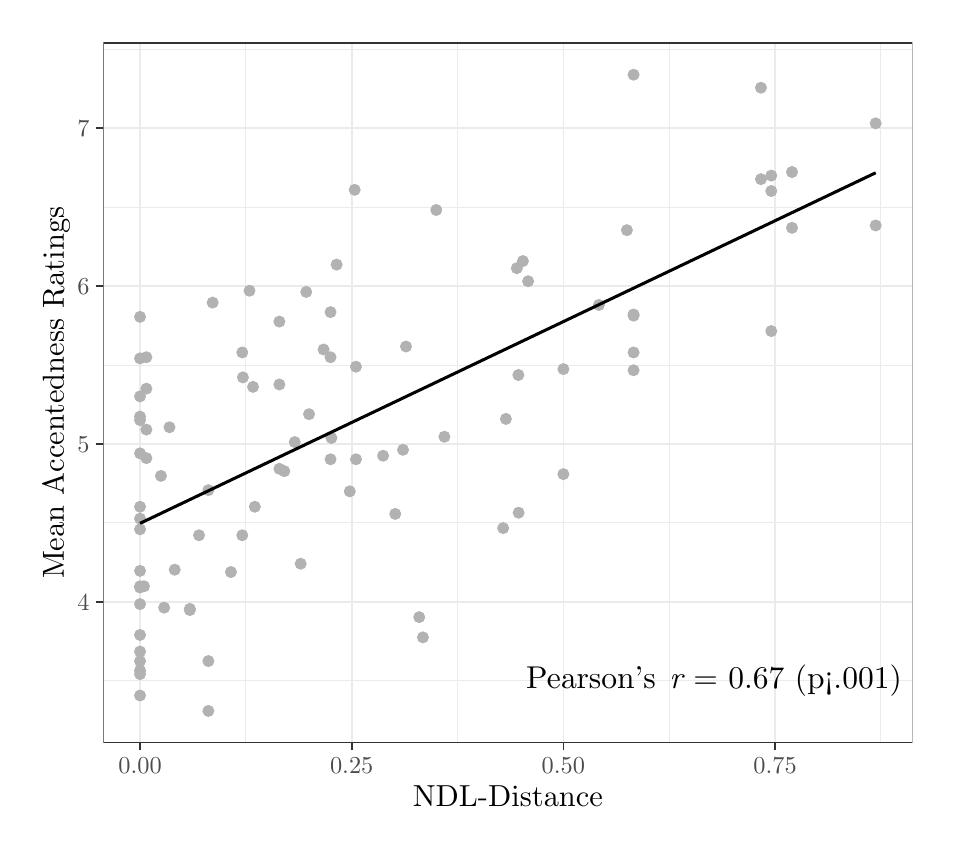
\begin{tikzpicture}[x=1pt,y=1pt]
\definecolor{fillColor}{RGB}{255,255,255}
\path[use as bounding box,fill=fillColor,fill opacity=0.00] (0,0) rectangle (325.21,289.08);
\begin{scope}
\path[clip] (  0.00,  0.00) rectangle (325.21,289.08);
\definecolor{drawColor}{RGB}{255,255,255}
\definecolor{fillColor}{RGB}{255,255,255}

\path[draw=drawColor,line width= 0.6pt,line join=round,line cap=round,fill=fillColor] (  0.00,  0.00) rectangle (325.21,289.08);
\end{scope}
\begin{scope}
\path[clip] ( 27.31, 30.69) rectangle (319.71,283.58);
\definecolor{fillColor}{RGB}{255,255,255}

\path[fill=fillColor] ( 27.31, 30.69) rectangle (319.71,283.58);
\definecolor{drawColor}{gray}{0.92}

\path[draw=drawColor,line width= 0.3pt,line join=round] ( 27.31, 53.12) --
	(319.71, 53.12);

\path[draw=drawColor,line width= 0.3pt,line join=round] ( 27.31,110.17) --
	(319.71,110.17);

\path[draw=drawColor,line width= 0.3pt,line join=round] ( 27.31,167.21) --
	(319.71,167.21);

\path[draw=drawColor,line width= 0.3pt,line join=round] ( 27.31,224.26) --
	(319.71,224.26);

\path[draw=drawColor,line width= 0.3pt,line join=round] ( 27.31,281.31) --
	(319.71,281.31);

\path[draw=drawColor,line width= 0.3pt,line join=round] ( 78.85, 30.69) --
	( 78.85,283.58);

\path[draw=drawColor,line width= 0.3pt,line join=round] (155.34, 30.69) --
	(155.34,283.58);

\path[draw=drawColor,line width= 0.3pt,line join=round] (231.82, 30.69) --
	(231.82,283.58);

\path[draw=drawColor,line width= 0.3pt,line join=round] (308.31, 30.69) --
	(308.31,283.58);

\path[draw=drawColor,line width= 0.6pt,line join=round] ( 27.31, 81.64) --
	(319.71, 81.64);

\path[draw=drawColor,line width= 0.6pt,line join=round] ( 27.31,138.69) --
	(319.71,138.69);

\path[draw=drawColor,line width= 0.6pt,line join=round] ( 27.31,195.74) --
	(319.71,195.74);

\path[draw=drawColor,line width= 0.6pt,line join=round] ( 27.31,252.78) --
	(319.71,252.78);

\path[draw=drawColor,line width= 0.6pt,line join=round] ( 40.60, 30.69) --
	( 40.60,283.58);

\path[draw=drawColor,line width= 0.6pt,line join=round] (117.09, 30.69) --
	(117.09,283.58);

\path[draw=drawColor,line width= 0.6pt,line join=round] (193.58, 30.69) --
	(193.58,283.58);

\path[draw=drawColor,line width= 0.6pt,line join=round] (270.07, 30.69) --
	(270.07,283.58);
\definecolor{drawColor}{gray}{0.70}
\definecolor{fillColor}{gray}{0.70}

\path[draw=drawColor,line width= 0.4pt,line join=round,line cap=round,fill=fillColor] ( 96.50,139.33) circle (  1.96);

\path[draw=drawColor,line width= 0.4pt,line join=round,line cap=round,fill=fillColor] (306.42,217.61) circle (  1.96);

\path[draw=drawColor,line width= 0.4pt,line join=round,line cap=round,fill=fillColor] (118.62,133.11) circle (  1.96);

\path[draw=drawColor,line width= 0.4pt,line join=round,line cap=round,fill=fillColor] ( 61.91,105.66) circle (  1.96);

\path[draw=drawColor,line width= 0.4pt,line join=round,line cap=round,fill=fillColor] (218.94,185.44) circle (  1.96);

\path[draw=drawColor,line width= 0.4pt,line join=round,line cap=round,fill=fillColor] ( 40.60, 60.20) circle (  1.96);

\path[draw=drawColor,line width= 0.4pt,line join=round,line cap=round,fill=fillColor] (136.70,173.86) circle (  1.96);

\path[draw=drawColor,line width= 0.4pt,line join=round,line cap=round,fill=fillColor] (218.94,171.72) circle (  1.96);

\path[draw=drawColor,line width= 0.4pt,line join=round,line cap=round,fill=fillColor] ( 58.60, 79.07) circle (  1.96);

\path[draw=drawColor,line width= 0.4pt,line join=round,line cap=round,fill=fillColor] (106.93,172.79) circle (  1.96);

\path[draw=drawColor,line width= 0.4pt,line join=round,line cap=round,fill=fillColor] (306.42,254.50) circle (  1.96);

\path[draw=drawColor,line width= 0.4pt,line join=round,line cap=round,fill=fillColor] ( 77.54,171.72) circle (  1.96);

\path[draw=drawColor,line width= 0.4pt,line join=round,line cap=round,fill=fillColor] ( 66.83,189.73) circle (  1.96);

\path[draw=drawColor,line width= 0.4pt,line join=round,line cap=round,fill=fillColor] (218.94,272.08) circle (  1.96);

\path[draw=drawColor,line width= 0.4pt,line join=round,line cap=round,fill=fillColor] ( 40.60,107.81) circle (  1.96);

\path[draw=drawColor,line width= 0.4pt,line join=round,line cap=round,fill=fillColor] (132.81,113.38) circle (  1.96);

\path[draw=drawColor,line width= 0.4pt,line join=round,line cap=round,fill=fillColor] ( 92.73,128.82) circle (  1.96);

\path[draw=drawColor,line width= 0.4pt,line join=round,line cap=round,fill=fillColor] (264.97,234.34) circle (  1.96);

\path[draw=drawColor,line width= 0.4pt,line join=round,line cap=round,fill=fillColor] ( 42.89,170.00) circle (  1.96);

\path[draw=drawColor,line width= 0.4pt,line join=round,line cap=round,fill=fillColor] ( 40.60,155.85) circle (  1.96);

\path[draw=drawColor,line width= 0.4pt,line join=round,line cap=round,fill=fillColor] (268.70,179.44) circle (  1.96);

\path[draw=drawColor,line width= 0.4pt,line join=round,line cap=round,fill=fillColor] ( 90.95,129.68) circle (  1.96);

\path[draw=drawColor,line width= 0.4pt,line join=round,line cap=round,fill=fillColor] ( 98.65, 95.37) circle (  1.96);

\path[draw=drawColor,line width= 0.4pt,line join=round,line cap=round,fill=fillColor] ( 90.95,160.14) circle (  1.96);

\path[draw=drawColor,line width= 0.4pt,line join=round,line cap=round,fill=fillColor] ( 40.60,184.58) circle (  1.96);

\path[draw=drawColor,line width= 0.4pt,line join=round,line cap=round,fill=fillColor] ( 82.08,115.96) circle (  1.96);

\path[draw=drawColor,line width= 0.4pt,line join=round,line cap=round,fill=fillColor] (141.48, 76.07) circle (  1.96);

\path[draw=drawColor,line width= 0.4pt,line join=round,line cap=round,fill=fillColor] ( 40.60, 56.76) circle (  1.96);

\path[draw=drawColor,line width= 0.4pt,line join=round,line cap=round,fill=fillColor] (177.40,113.81) circle (  1.96);

\path[draw=drawColor,line width= 0.4pt,line join=round,line cap=round,fill=fillColor] ( 40.60, 87.22) circle (  1.96);

\path[draw=drawColor,line width= 0.4pt,line join=round,line cap=round,fill=fillColor] (135.63,136.54) circle (  1.96);

\path[draw=drawColor,line width= 0.4pt,line join=round,line cap=round,fill=fillColor] (177.31,163.57) circle (  1.96);

\path[draw=drawColor,line width= 0.4pt,line join=round,line cap=round,fill=fillColor] (216.53,215.90) circle (  1.96);

\path[draw=drawColor,line width= 0.4pt,line join=round,line cap=round,fill=fillColor] ( 40.60, 80.78) circle (  1.96);

\path[draw=drawColor,line width= 0.4pt,line join=round,line cap=round,fill=fillColor] ( 53.13, 93.22) circle (  1.96);

\path[draw=drawColor,line width= 0.4pt,line join=round,line cap=round,fill=fillColor] ( 40.60,111.67) circle (  1.96);

\path[draw=drawColor,line width= 0.4pt,line join=round,line cap=round,fill=fillColor] ( 49.31, 79.50) circle (  1.96);

\path[draw=drawColor,line width= 0.4pt,line join=round,line cap=round,fill=fillColor] (180.83,197.45) circle (  1.96);

\path[draw=drawColor,line width= 0.4pt,line join=round,line cap=round,fill=fillColor] (109.44,186.30) circle (  1.96);

\path[draw=drawColor,line width= 0.4pt,line join=round,line cap=round,fill=fillColor] (147.64,223.19) circle (  1.96);

\path[draw=drawColor,line width= 0.4pt,line join=round,line cap=round,fill=fillColor] (218.94,165.28) circle (  1.96);

\path[draw=drawColor,line width= 0.4pt,line join=round,line cap=round,fill=fillColor] (268.70,235.63) circle (  1.96);

\path[draw=drawColor,line width= 0.4pt,line join=round,line cap=round,fill=fillColor] (118.62,166.57) circle (  1.96);

\path[draw=drawColor,line width= 0.4pt,line join=round,line cap=round,fill=fillColor] ( 81.43,159.28) circle (  1.96);

\path[draw=drawColor,line width= 0.4pt,line join=round,line cap=round,fill=fillColor] (118.16,230.48) circle (  1.96);

\path[draw=drawColor,line width= 0.4pt,line join=round,line cap=round,fill=fillColor] (109.44,133.11) circle (  1.96);

\path[draw=drawColor,line width= 0.4pt,line join=round,line cap=round,fill=fillColor] ( 58.60, 78.64) circle (  1.96);

\path[draw=drawColor,line width= 0.4pt,line join=round,line cap=round,fill=fillColor] ( 40.60, 47.76) circle (  1.96);

\path[draw=drawColor,line width= 0.4pt,line join=round,line cap=round,fill=fillColor] (109.44,170.00) circle (  1.96);

\path[draw=drawColor,line width= 0.4pt,line join=round,line cap=round,fill=fillColor] ( 42.02, 87.22) circle (  1.96);

\path[draw=drawColor,line width= 0.4pt,line join=round,line cap=round,fill=fillColor] ( 40.60,148.55) circle (  1.96);

\path[draw=drawColor,line width= 0.4pt,line join=round,line cap=round,fill=fillColor] (276.19,236.91) circle (  1.96);

\path[draw=drawColor,line width= 0.4pt,line join=round,line cap=round,fill=fillColor] (206.42,188.87) circle (  1.96);

\path[draw=drawColor,line width= 0.4pt,line join=round,line cap=round,fill=fillColor] ( 77.54,105.66) circle (  1.96);

\path[draw=drawColor,line width= 0.4pt,line join=round,line cap=round,fill=fillColor] (176.75,202.17) circle (  1.96);

\path[draw=drawColor,line width= 0.4pt,line join=round,line cap=round,fill=fillColor] (101.66,149.41) circle (  1.96);

\path[draw=drawColor,line width= 0.4pt,line join=round,line cap=round,fill=fillColor] (193.58,127.75) circle (  1.96);

\path[draw=drawColor,line width= 0.4pt,line join=round,line cap=round,fill=fillColor] ( 40.60,115.96) circle (  1.96);

\path[draw=drawColor,line width= 0.4pt,line join=round,line cap=round,fill=fillColor] (116.39,121.53) circle (  1.96);

\path[draw=drawColor,line width= 0.4pt,line join=round,line cap=round,fill=fillColor] ( 40.60, 69.63) circle (  1.96);

\path[draw=drawColor,line width= 0.4pt,line join=round,line cap=round,fill=fillColor] ( 42.89,133.54) circle (  1.96);

\path[draw=drawColor,line width= 0.4pt,line join=round,line cap=round,fill=fillColor] (128.44,134.40) circle (  1.96);

\path[draw=drawColor,line width= 0.4pt,line join=round,line cap=round,fill=fillColor] (172.80,147.70) circle (  1.96);

\path[draw=drawColor,line width= 0.4pt,line join=round,line cap=round,fill=fillColor] ( 40.60,135.26) circle (  1.96);

\path[draw=drawColor,line width= 0.4pt,line join=round,line cap=round,fill=fillColor] ( 40.60,169.57) circle (  1.96);

\path[draw=drawColor,line width= 0.4pt,line join=round,line cap=round,fill=fillColor] (111.63,203.46) circle (  1.96);

\path[draw=drawColor,line width= 0.4pt,line join=round,line cap=round,fill=fillColor] ( 90.95,182.87) circle (  1.96);

\path[draw=drawColor,line width= 0.4pt,line join=round,line cap=round,fill=fillColor] (100.65,193.59) circle (  1.96);

\path[draw=drawColor,line width= 0.4pt,line join=round,line cap=round,fill=fillColor] (218.94,185.01) circle (  1.96);

\path[draw=drawColor,line width= 0.4pt,line join=round,line cap=round,fill=fillColor] ( 73.45, 92.37) circle (  1.96);

\path[draw=drawColor,line width= 0.4pt,line join=round,line cap=round,fill=fillColor] ( 40.60, 86.79) circle (  1.96);

\path[draw=drawColor,line width= 0.4pt,line join=round,line cap=round,fill=fillColor] ( 48.16,127.11) circle (  1.96);

\path[draw=drawColor,line width= 0.4pt,line join=round,line cap=round,fill=fillColor] (142.82, 68.77) circle (  1.96);

\path[draw=drawColor,line width= 0.4pt,line join=round,line cap=round,fill=fillColor] (264.97,267.37) circle (  1.96);

\path[draw=drawColor,line width= 0.4pt,line join=round,line cap=round,fill=fillColor] ( 80.15,194.02) circle (  1.96);

\path[draw=drawColor,line width= 0.4pt,line join=round,line cap=round,fill=fillColor] ( 40.60, 63.63) circle (  1.96);

\path[draw=drawColor,line width= 0.4pt,line join=round,line cap=round,fill=fillColor] ( 40.60, 92.79) circle (  1.96);

\path[draw=drawColor,line width= 0.4pt,line join=round,line cap=round,fill=fillColor] ( 40.60,147.27) circle (  1.96);

\path[draw=drawColor,line width= 0.4pt,line join=round,line cap=round,fill=fillColor] ( 77.78,162.71) circle (  1.96);

\path[draw=drawColor,line width= 0.4pt,line join=round,line cap=round,fill=fillColor] (171.82,108.24) circle (  1.96);

\path[draw=drawColor,line width= 0.4pt,line join=round,line cap=round,fill=fillColor] ( 42.89,143.84) circle (  1.96);

\path[draw=drawColor,line width= 0.4pt,line join=round,line cap=round,fill=fillColor] ( 65.29, 60.20) circle (  1.96);

\path[draw=drawColor,line width= 0.4pt,line join=round,line cap=round,fill=fillColor] (276.19,216.75) circle (  1.96);

\path[draw=drawColor,line width= 0.4pt,line join=round,line cap=round,fill=fillColor] (193.58,165.71) circle (  1.96);

\path[draw=drawColor,line width= 0.4pt,line join=round,line cap=round,fill=fillColor] ( 42.89,158.63) circle (  1.96);

\path[draw=drawColor,line width= 0.4pt,line join=round,line cap=round,fill=fillColor] ( 40.60, 55.48) circle (  1.96);

\path[draw=drawColor,line width= 0.4pt,line join=round,line cap=round,fill=fillColor] (178.95,204.74) circle (  1.96);

\path[draw=drawColor,line width= 0.4pt,line join=round,line cap=round,fill=fillColor] ( 51.25,144.69) circle (  1.96);

\path[draw=drawColor,line width= 0.4pt,line join=round,line cap=round,fill=fillColor] (268.70,230.05) circle (  1.96);

\path[draw=drawColor,line width= 0.4pt,line join=round,line cap=round,fill=fillColor] (150.58,141.26) circle (  1.96);

\path[draw=drawColor,line width= 0.4pt,line join=round,line cap=round,fill=fillColor] ( 65.29, 42.18) circle (  1.96);

\path[draw=drawColor,line width= 0.4pt,line join=round,line cap=round,fill=fillColor] ( 65.29,121.96) circle (  1.96);

\path[draw=drawColor,line width= 0.4pt,line join=round,line cap=round,fill=fillColor] (109.76,140.83) circle (  1.96);
\definecolor{drawColor}{RGB}{0,0,0}

\path[draw=drawColor,line width= 1.1pt,line join=round] ( 40.60,109.96) --
	( 43.97,111.57) --
	( 47.33,113.17) --
	( 50.70,114.78) --
	( 54.06,116.38) --
	( 57.43,117.98) --
	( 60.79,119.59) --
	( 64.16,121.19) --
	( 67.52,122.79) --
	( 70.89,124.40) --
	( 74.25,126.00) --
	( 77.62,127.60) --
	( 80.98,129.21) --
	( 84.35,130.81) --
	( 87.71,132.41) --
	( 91.08,134.02) --
	( 94.44,135.62) --
	( 97.81,137.22) --
	(101.17,138.83) --
	(104.54,140.43) --
	(107.90,142.03) --
	(111.27,143.64) --
	(114.63,145.24) --
	(117.99,146.85) --
	(121.36,148.45) --
	(124.72,150.05) --
	(128.09,151.66) --
	(131.45,153.26) --
	(134.82,154.86) --
	(138.18,156.47) --
	(141.55,158.07) --
	(144.91,159.67) --
	(148.28,161.28) --
	(151.64,162.88) --
	(155.01,164.48) --
	(158.37,166.09) --
	(161.74,167.69) --
	(165.10,169.29) --
	(168.47,170.90) --
	(171.83,172.50) --
	(175.20,174.10) --
	(178.56,175.71) --
	(181.93,177.31) --
	(185.29,178.92) --
	(188.66,180.52) --
	(192.02,182.12) --
	(195.39,183.73) --
	(198.75,185.33) --
	(202.11,186.93) --
	(205.48,188.54) --
	(208.84,190.14) --
	(212.21,191.74) --
	(215.57,193.35) --
	(218.94,194.95) --
	(222.30,196.55) --
	(225.67,198.16) --
	(229.03,199.76) --
	(232.40,201.36) --
	(235.76,202.97) --
	(239.13,204.57) --
	(242.49,206.17) --
	(245.86,207.78) --
	(249.22,209.38) --
	(252.59,210.99) --
	(255.95,212.59) --
	(259.32,214.19) --
	(262.68,215.80) --
	(266.05,217.40) --
	(269.41,219.00) --
	(272.78,220.61) --
	(276.14,222.21) --
	(279.51,223.81) --
	(282.87,225.42) --
	(286.24,227.02) --
	(289.60,228.62) --
	(292.96,230.23) --
	(296.33,231.83) --
	(299.69,233.43) --
	(303.06,235.04) --
	(306.42,236.64);

\node[text=drawColor,anchor=base west,inner sep=0pt, outer sep=0pt, scale=  1.14] at (180.13, 50.27) {Pearson's};

\node[text=drawColor,anchor=base west,inner sep=0pt, outer sep=0pt, scale=  1.14] at (231.90, 50.27) {\itshape  r};

\node[text=drawColor,anchor=base west,inner sep=0pt, outer sep=0pt, scale=  1.14] at (240.51, 50.27) { = 0.67 (p<.001)};
\definecolor{drawColor}{gray}{0.20}

\path[draw=drawColor,line width= 0.6pt,line join=round,line cap=round] ( 27.31, 30.69) rectangle (319.71,283.58);
\end{scope}
\begin{scope}
\path[clip] (  0.00,  0.00) rectangle (325.21,289.08);
\definecolor{drawColor}{gray}{0.30}

\node[text=drawColor,anchor=base east,inner sep=0pt, outer sep=0pt, scale=  0.88] at ( 22.36, 78.61) {4};

\node[text=drawColor,anchor=base east,inner sep=0pt, outer sep=0pt, scale=  0.88] at ( 22.36,135.66) {5};

\node[text=drawColor,anchor=base east,inner sep=0pt, outer sep=0pt, scale=  0.88] at ( 22.36,192.71) {6};

\node[text=drawColor,anchor=base east,inner sep=0pt, outer sep=0pt, scale=  0.88] at ( 22.36,249.75) {7};
\end{scope}
\begin{scope}
\path[clip] (  0.00,  0.00) rectangle (325.21,289.08);
\definecolor{drawColor}{gray}{0.20}

\path[draw=drawColor,line width= 0.6pt,line join=round] ( 24.56, 81.64) --
	( 27.31, 81.64);

\path[draw=drawColor,line width= 0.6pt,line join=round] ( 24.56,138.69) --
	( 27.31,138.69);

\path[draw=drawColor,line width= 0.6pt,line join=round] ( 24.56,195.74) --
	( 27.31,195.74);

\path[draw=drawColor,line width= 0.6pt,line join=round] ( 24.56,252.78) --
	( 27.31,252.78);
\end{scope}
\begin{scope}
\path[clip] (  0.00,  0.00) rectangle (325.21,289.08);
\definecolor{drawColor}{gray}{0.20}

\path[draw=drawColor,line width= 0.6pt,line join=round] ( 40.60, 27.94) --
	( 40.60, 30.69);

\path[draw=drawColor,line width= 0.6pt,line join=round] (117.09, 27.94) --
	(117.09, 30.69);

\path[draw=drawColor,line width= 0.6pt,line join=round] (193.58, 27.94) --
	(193.58, 30.69);

\path[draw=drawColor,line width= 0.6pt,line join=round] (270.07, 27.94) --
	(270.07, 30.69);
\end{scope}
\begin{scope}
\path[clip] (  0.00,  0.00) rectangle (325.21,289.08);
\definecolor{drawColor}{gray}{0.30}

\node[text=drawColor,anchor=base,inner sep=0pt, outer sep=0pt, scale=  0.88] at ( 40.60, 19.68) {0.00};

\node[text=drawColor,anchor=base,inner sep=0pt, outer sep=0pt, scale=  0.88] at (117.09, 19.68) {0.25};

\node[text=drawColor,anchor=base,inner sep=0pt, outer sep=0pt, scale=  0.88] at (193.58, 19.68) {0.50};

\node[text=drawColor,anchor=base,inner sep=0pt, outer sep=0pt, scale=  0.88] at (270.07, 19.68) {0.75};
\end{scope}
\begin{scope}
\path[clip] (  0.00,  0.00) rectangle (325.21,289.08);
\definecolor{drawColor}{RGB}{0,0,0}

\node[text=drawColor,anchor=base,inner sep=0pt, outer sep=0pt, scale=  1.10] at (173.51,  7.64) {NDL-Distance};
\end{scope}
\begin{scope}
\path[clip] (  0.00,  0.00) rectangle (325.21,289.08);
\definecolor{drawColor}{RGB}{0,0,0}

\node[text=drawColor,rotate= 90.00,anchor=base,inner sep=0pt, outer sep=0pt, scale=  1.10] at ( 13.08,157.13) {Mean Accentedness Ratings};
\end{scope}
\end{tikzpicture}

	%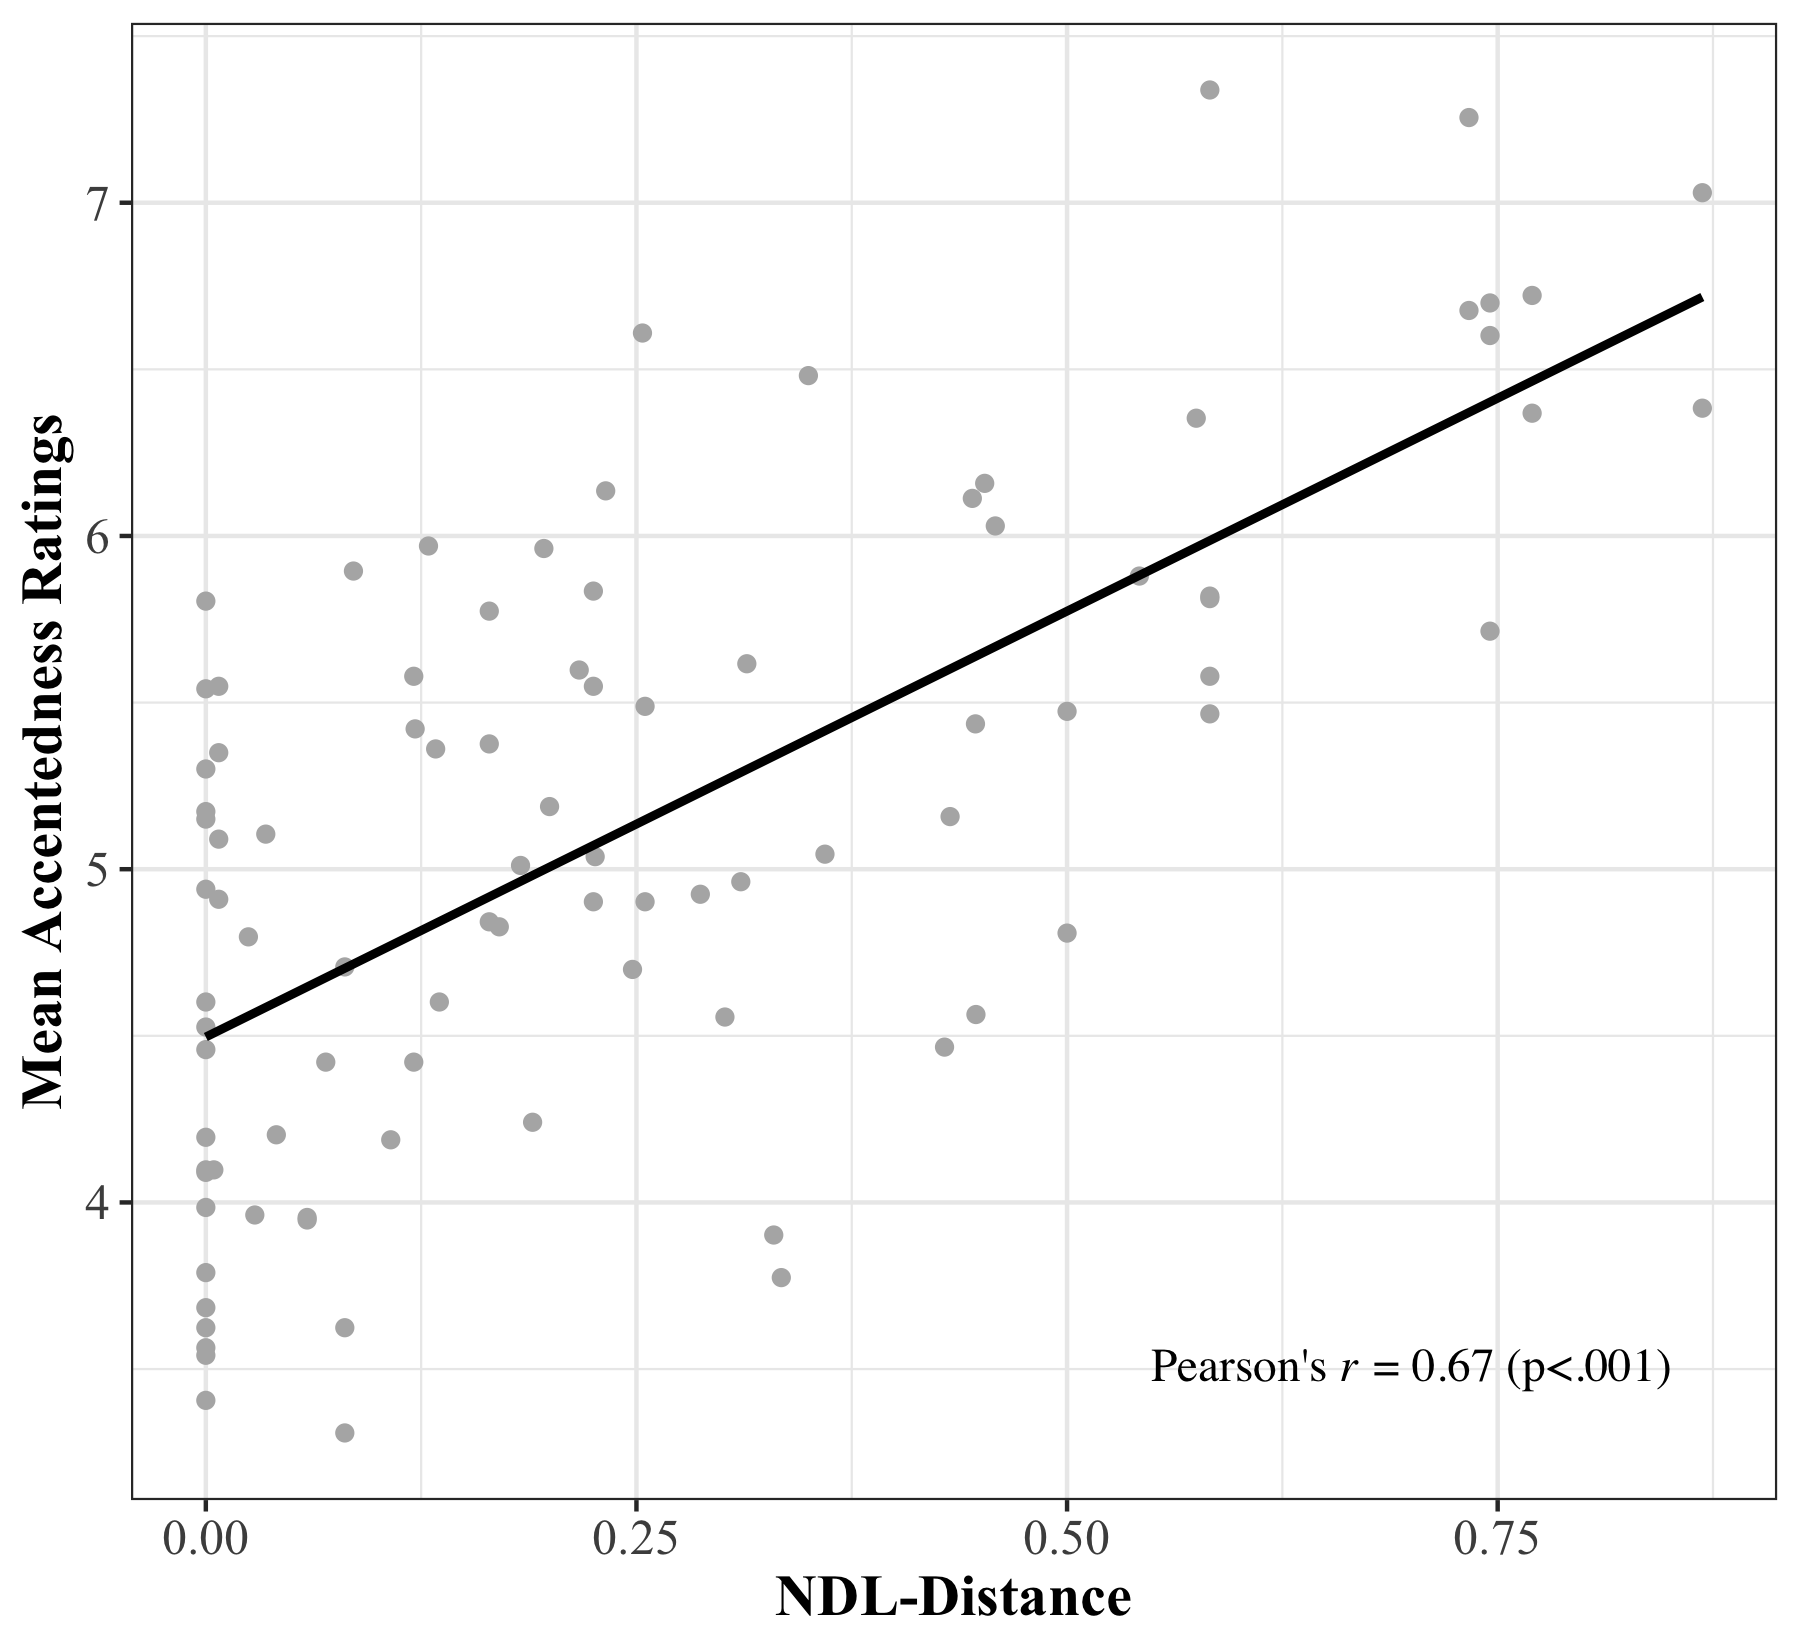
\includegraphics[width=0.75\textwidth]{figures/ndl/all.png}
    \caption{Relationship between Accentedness and NDL-Distance}
    \label{fig:all}
  \figSpace
\end{figure}

Overall, there is a clear positive relationship between the accentedness ratings and the NDL-distances (Pearson’s r = .67, p <.001). This result generally agrees with the prediction that the larger the NDL-distance between an L2 stimulus and its corresponding L1 productions, the more accented the L2 stimulus will be judged.

\subsubsection{Types of Mismatches}

Linear mixed-effects regression models were constructed to investigate the effects of the four types of stimuli (i.e., consonant vs. syllable vs. vowel vs. match), while controlling for NDL-distances. Rating data from Experiment 2 were used for the analysis. Accentednss ratings were the dependent variable. Helmert-contrast-coding was again performed on the “types of stimuli” variable to create three contrasts. The first contrast compares stimuli with consonant mismatches and stimuli with syllable mismatches, the second contrast compares vowel mismatches with consonant and syllable mismatches, and the third contrast compares the match stimuli with the three types of mismatch stimuli. The three contrasts, trial numbers and NDL-distances for the stimuli were entered as fixed effects. Two-way and three-way interactions of the fixed effects were also entered as fixed effects. Raters and stimuli were entered as random effects.

Model comparisons using likelihood ratio tests showed that (1) NDL-distances significantly contributed to model fit ($\beta$ = 1.74, χ2 = 8.79, p<.01), showing that the degree of dissimilarity between L1 and L2 speech samples could have affected accentedness perception; (2) trial number contributed significantly to model fit ($\beta$ = 0.6, χ2 = 72.24, p<.001), showing that the accentedness ratings increased overtime; and (3) the three contrasts did not contribute significantly to model fit, showing that accentedness differences between the four types of stimuli diminished once NDL-distances were controlled for.

To further investigate the interactions between NDL-distances and the types of mismatches, mean accentedness ratings of each type of mismatch were plotted against NDL-distances. Figure \ref{fig:con} demonstrates the relationship between NDL-distances and accentedness ratings of stimuli with consonant and syllable mismatches.

\begin{figure}[!h]
  \figSpace
    \centering
    % Created by tikzDevice version 0.12.3 on 2019-11-25 15:09:07
% !TEX encoding = UTF-8 Unicode
\begin{tikzpicture}[x=1pt,y=1pt]
\definecolor{fillColor}{RGB}{255,255,255}
\path[use as bounding box,fill=fillColor,fill opacity=0.00] (0,0) rectangle (325.21,289.08);
\begin{scope}
\path[clip] (  0.00,  0.00) rectangle (325.21,289.08);
\definecolor{drawColor}{RGB}{255,255,255}
\definecolor{fillColor}{RGB}{255,255,255}

\path[draw=drawColor,line width= 0.6pt,line join=round,line cap=round,fill=fillColor] (  0.00,  0.00) rectangle (325.21,289.08);
\end{scope}
\begin{scope}
\path[clip] ( 27.31, 30.69) rectangle (319.71,267.01);
\definecolor{fillColor}{RGB}{255,255,255}

\path[fill=fillColor] ( 27.31, 30.69) rectangle (319.71,267.01);
\definecolor{drawColor}{gray}{0.92}

\path[draw=drawColor,line width= 0.3pt,line join=round] ( 27.31, 65.30) --
	(319.71, 65.30);

\path[draw=drawColor,line width= 0.3pt,line join=round] ( 27.31,113.04) --
	(319.71,113.04);

\path[draw=drawColor,line width= 0.3pt,line join=round] ( 27.31,160.78) --
	(319.71,160.78);

\path[draw=drawColor,line width= 0.3pt,line join=round] ( 27.31,208.52) --
	(319.71,208.52);

\path[draw=drawColor,line width= 0.3pt,line join=round] ( 27.31,256.27) --
	(319.71,256.27);

\path[draw=drawColor,line width= 0.3pt,line join=round] ( 73.83, 30.69) --
	( 73.83,267.01);

\path[draw=drawColor,line width= 0.3pt,line join=round] (140.29, 30.69) --
	(140.29,267.01);

\path[draw=drawColor,line width= 0.3pt,line join=round] (206.74, 30.69) --
	(206.74,267.01);

\path[draw=drawColor,line width= 0.3pt,line join=round] (273.20, 30.69) --
	(273.20,267.01);

\path[draw=drawColor,line width= 0.6pt,line join=round] ( 27.31, 41.43) --
	(319.71, 41.43);

\path[draw=drawColor,line width= 0.6pt,line join=round] ( 27.31, 89.17) --
	(319.71, 89.17);

\path[draw=drawColor,line width= 0.6pt,line join=round] ( 27.31,136.91) --
	(319.71,136.91);

\path[draw=drawColor,line width= 0.6pt,line join=round] ( 27.31,184.65) --
	(319.71,184.65);

\path[draw=drawColor,line width= 0.6pt,line join=round] ( 27.31,232.40) --
	(319.71,232.40);

\path[draw=drawColor,line width= 0.6pt,line join=round] ( 40.60, 30.69) --
	( 40.60,267.01);

\path[draw=drawColor,line width= 0.6pt,line join=round] (107.06, 30.69) --
	(107.06,267.01);

\path[draw=drawColor,line width= 0.6pt,line join=round] (173.51, 30.69) --
	(173.51,267.01);

\path[draw=drawColor,line width= 0.6pt,line join=round] (239.97, 30.69) --
	(239.97,267.01);

\path[draw=drawColor,line width= 0.6pt,line join=round] (306.42, 30.69) --
	(306.42,267.01);
\definecolor{fillColor}{gray}{0.10}

\path[fill=fillColor] ( 89.17,137.45) circle (  1.96);

\path[fill=fillColor] (271.56,202.96) circle (  1.96);

\path[fill=fillColor] ( 59.11,109.27) circle (  1.96);

\path[fill=fillColor] (195.55,176.04) circle (  1.96);

\path[fill=fillColor] (195.55,164.55) circle (  1.96);

\path[fill=fillColor] (271.56,233.83) circle (  1.96);

\path[fill=fillColor] ( 72.69,164.55) circle (  1.96);

\path[fill=fillColor] (195.55,248.55) circle (  1.96);

\path[fill=fillColor] (193.45,201.52) circle (  1.96);

\path[fill=fillColor] (133.60,207.63) circle (  1.96);

\path[fill=fillColor] (195.55,159.17) circle (  1.96);

\path[fill=fillColor] (107.99,213.73) circle (  1.96);

\path[fill=fillColor] (184.67,178.91) circle (  1.96);

\path[fill=fillColor] ( 72.69,109.27) circle (  1.96);

\path[fill=fillColor] (116.92,133.32) circle (  1.96);

\path[fill=fillColor] (155.46,144.45) circle (  1.96);

\path[fill=fillColor] (102.31,191.11) circle (  1.96);

\path[fill=fillColor] (195.55,175.68) circle (  1.96);

\path[fill=fillColor] ( 72.91,157.01) circle (  1.96);

\path[fill=fillColor] (154.60,111.43) circle (  1.96);

\path[fill=fillColor] (160.80,192.19) circle (  1.96);

\path[fill=fillColor] (100.69,138.71) circle (  1.96);
\definecolor{drawColor}{RGB}{26,26,26}

\node[text=drawColor,text opacity=0.80,anchor=base,inner sep=0pt, outer sep=0pt, scale=  0.85] at ( 89.17,130.57) {kʰ$\rightarrow$k};

\node[text=drawColor,text opacity=0.80,anchor=base,inner sep=0pt, outer sep=0pt, scale=  0.85] at (271.56,197.08) {pʰl$\rightarrow$pl};

\node[text=drawColor,text opacity=0.80,anchor=base,inner sep=0pt, outer sep=0pt, scale=  0.85] at ( 59.11,103.39) {pʰl$\rightarrow$pl};

\node[text=drawColor,text opacity=0.80,anchor=base,inner sep=0pt, outer sep=0pt, scale=  0.85] at (195.55,170.16) {ɹ$\rightarrow$r};

\node[text=drawColor,text opacity=0.80,anchor=base,inner sep=0pt, outer sep=0pt, scale=  0.85] at (195.55,158.67) {ɹ$\rightarrow$r};

\node[text=drawColor,text opacity=0.80,anchor=base,inner sep=0pt, outer sep=0pt, scale=  0.85] at (271.56,227.95) {pʰl$\rightarrow$pl};

\node[text=drawColor,text opacity=0.80,anchor=base,inner sep=0pt, outer sep=0pt, scale=  0.85] at ( 72.69,158.67) {θ$\rightarrow$t̪};

\node[text=drawColor,text opacity=0.80,anchor=base,inner sep=0pt, outer sep=0pt, scale=  0.85] at (195.55,242.67) {ɹ$\rightarrow$r};

\node[text=drawColor,text opacity=0.80,anchor=base,inner sep=0pt, outer sep=0pt, scale=  0.85] at (193.45,195.65) {θ$\rightarrow$st};

\node[text=drawColor,text opacity=0.80,anchor=base,inner sep=0pt, outer sep=0pt, scale=  0.85] at (133.60,201.75) {pʰl$\rightarrow$pʰll};

\node[text=drawColor,text opacity=0.80,anchor=base,inner sep=0pt, outer sep=0pt, scale=  0.85] at (195.55,153.29) {ɹ$\rightarrow$r};

\node[text=drawColor,text opacity=0.80,anchor=base,inner sep=0pt, outer sep=0pt, scale=  0.85] at (107.99,207.85) {pʰl$\rightarrow$pʰɾ};

\node[text=drawColor,text opacity=0.80,anchor=base,inner sep=0pt, outer sep=0pt, scale=  0.85] at (184.67,173.03) {spũnz$\rightarrow$spũnʃ};

\node[text=drawColor,text opacity=0.80,anchor=base,inner sep=0pt, outer sep=0pt, scale=  0.85] at ( 72.69,103.39) {θ$\rightarrow$t̪};

\node[text=drawColor,text opacity=0.80,anchor=base,inner sep=0pt, outer sep=0pt, scale=  0.85] at (116.92,127.44) {θ$\rightarrow$f};

\node[text=drawColor,text opacity=0.80,anchor=base,inner sep=0pt, outer sep=0pt, scale=  0.85] at (155.46,138.57) {sm$\rightarrow$zm};

\node[text=drawColor,text opacity=0.80,anchor=base,inner sep=0pt, outer sep=0pt, scale=  0.85] at (102.31,185.24) {smɑl$\rightarrow$smɑɭ};

\node[text=drawColor,text opacity=0.80,anchor=base,inner sep=0pt, outer sep=0pt, scale=  0.85] at (195.55,169.80) {ɹ$\rightarrow$r};

\node[text=drawColor,text opacity=0.80,anchor=base,inner sep=0pt, outer sep=0pt, scale=  0.85] at ( 72.91,151.13) {θ$\rightarrow$t̪};

\node[text=drawColor,text opacity=0.80,anchor=base,inner sep=0pt, outer sep=0pt, scale=  0.85] at (154.60,105.55) {sp$\rightarrow$spʰ};

\node[text=drawColor,text opacity=0.80,anchor=base,inner sep=0pt, outer sep=0pt, scale=  0.85] at (160.80,186.31) {sp$\rightarrow$spʰ};

\node[text=drawColor,text opacity=0.80,anchor=base,inner sep=0pt, outer sep=0pt, scale=  0.85] at (100.69,138.83) {pʰliz$\rightarrow$pʰlis};
\definecolor{drawColor}{RGB}{0,0,0}

\path[draw=drawColor,line width= 1.1pt,line join=round] ( 59.11,137.33) --
	( 61.80,138.32) --
	( 64.49,139.30) --
	( 67.18,140.28) --
	( 69.87,141.26) --
	( 72.56,142.25) --
	( 75.25,143.23) --
	( 77.94,144.21) --
	( 80.63,145.20) --
	( 83.32,146.18) --
	( 86.00,147.16) --
	( 88.69,148.14) --
	( 91.38,149.13) --
	( 94.07,150.11) --
	( 96.76,151.09) --
	( 99.45,152.08) --
	(102.14,153.06) --
	(104.83,154.04) --
	(107.52,155.02) --
	(110.21,156.01) --
	(112.90,156.99) --
	(115.59,157.97) --
	(118.27,158.95) --
	(120.96,159.94) --
	(123.65,160.92) --
	(126.34,161.90) --
	(129.03,162.89) --
	(131.72,163.87) --
	(134.41,164.85) --
	(137.10,165.83) --
	(139.79,166.82) --
	(142.48,167.80) --
	(145.17,168.78) --
	(147.85,169.77) --
	(150.54,170.75) --
	(153.23,171.73) --
	(155.92,172.71) --
	(158.61,173.70) --
	(161.30,174.68) --
	(163.99,175.66) --
	(166.68,176.65) --
	(169.37,177.63) --
	(172.06,178.61) --
	(174.75,179.59) --
	(177.44,180.58) --
	(180.12,181.56) --
	(182.81,182.54) --
	(185.50,183.53) --
	(188.19,184.51) --
	(190.88,185.49) --
	(193.57,186.47) --
	(196.26,187.46) --
	(198.95,188.44) --
	(201.64,189.42) --
	(204.33,190.41) --
	(207.02,191.39) --
	(209.71,192.37) --
	(212.39,193.35) --
	(215.08,194.34) --
	(217.77,195.32) --
	(220.46,196.30) --
	(223.15,197.28) --
	(225.84,198.27) --
	(228.53,199.25) --
	(231.22,200.23) --
	(233.91,201.22) --
	(236.60,202.20) --
	(239.29,203.18) --
	(241.97,204.16) --
	(244.66,205.15) --
	(247.35,206.13) --
	(250.04,207.11) --
	(252.73,208.10) --
	(255.42,209.08) --
	(258.11,210.06) --
	(260.80,211.04) --
	(263.49,212.03) --
	(266.18,213.01) --
	(268.87,213.99) --
	(271.56,214.98);

\node[text=drawColor,anchor=base west,inner sep=0pt, outer sep=0pt, scale=  1.14] at (155.88, 62.45) {Pearson's};

\node[text=drawColor,anchor=base west,inner sep=0pt, outer sep=0pt, scale=  1.14] at (207.66, 62.45) {\itshape  r};

\node[text=drawColor,anchor=base west,inner sep=0pt, outer sep=0pt, scale=  1.14] at (217.26, 62.45) { = 0.58 (p<.01)};
\definecolor{drawColor}{gray}{0.20}

\path[draw=drawColor,line width= 0.6pt,line join=round,line cap=round] ( 27.31, 30.69) rectangle (319.71,267.01);
\end{scope}
\begin{scope}
\path[clip] ( 27.31,267.01) rectangle (319.71,283.58);
\definecolor{drawColor}{gray}{0.20}
\definecolor{fillColor}{gray}{0.85}

\path[draw=drawColor,line width= 0.6pt,line join=round,line cap=round,fill=fillColor] ( 27.31,267.01) rectangle (319.71,283.58);
\definecolor{drawColor}{gray}{0.10}

\node[text=drawColor,anchor=base,inner sep=0pt, outer sep=0pt, scale=  0.88] at (173.51,272.26) {Consonant};
\end{scope}
\begin{scope}
\path[clip] (  0.00,  0.00) rectangle (325.21,289.08);
\definecolor{drawColor}{gray}{0.20}

\path[draw=drawColor,line width= 0.6pt,line join=round] ( 40.60, 27.94) --
	( 40.60, 30.69);

\path[draw=drawColor,line width= 0.6pt,line join=round] (107.06, 27.94) --
	(107.06, 30.69);

\path[draw=drawColor,line width= 0.6pt,line join=round] (173.51, 27.94) --
	(173.51, 30.69);

\path[draw=drawColor,line width= 0.6pt,line join=round] (239.97, 27.94) --
	(239.97, 30.69);

\path[draw=drawColor,line width= 0.6pt,line join=round] (306.42, 27.94) --
	(306.42, 30.69);
\end{scope}
\begin{scope}
\path[clip] (  0.00,  0.00) rectangle (325.21,289.08);
\definecolor{drawColor}{gray}{0.30}

\node[text=drawColor,anchor=base,inner sep=0pt, outer sep=0pt, scale=  0.88] at ( 40.60, 19.68) {0.00};

\node[text=drawColor,anchor=base,inner sep=0pt, outer sep=0pt, scale=  0.88] at (107.06, 19.68) {0.25};

\node[text=drawColor,anchor=base,inner sep=0pt, outer sep=0pt, scale=  0.88] at (173.51, 19.68) {0.50};

\node[text=drawColor,anchor=base,inner sep=0pt, outer sep=0pt, scale=  0.88] at (239.97, 19.68) {0.75};

\node[text=drawColor,anchor=base,inner sep=0pt, outer sep=0pt, scale=  0.88] at (306.42, 19.68) {1.00};
\end{scope}
\begin{scope}
\path[clip] (  0.00,  0.00) rectangle (325.21,289.08);
\definecolor{drawColor}{gray}{0.30}

\node[text=drawColor,anchor=base east,inner sep=0pt, outer sep=0pt, scale=  0.88] at ( 22.36, 38.40) {3};

\node[text=drawColor,anchor=base east,inner sep=0pt, outer sep=0pt, scale=  0.88] at ( 22.36, 86.14) {4};

\node[text=drawColor,anchor=base east,inner sep=0pt, outer sep=0pt, scale=  0.88] at ( 22.36,133.88) {5};

\node[text=drawColor,anchor=base east,inner sep=0pt, outer sep=0pt, scale=  0.88] at ( 22.36,181.62) {6};

\node[text=drawColor,anchor=base east,inner sep=0pt, outer sep=0pt, scale=  0.88] at ( 22.36,229.37) {7};
\end{scope}
\begin{scope}
\path[clip] (  0.00,  0.00) rectangle (325.21,289.08);
\definecolor{drawColor}{gray}{0.20}

\path[draw=drawColor,line width= 0.6pt,line join=round] ( 24.56, 41.43) --
	( 27.31, 41.43);

\path[draw=drawColor,line width= 0.6pt,line join=round] ( 24.56, 89.17) --
	( 27.31, 89.17);

\path[draw=drawColor,line width= 0.6pt,line join=round] ( 24.56,136.91) --
	( 27.31,136.91);

\path[draw=drawColor,line width= 0.6pt,line join=round] ( 24.56,184.65) --
	( 27.31,184.65);

\path[draw=drawColor,line width= 0.6pt,line join=round] ( 24.56,232.40) --
	( 27.31,232.40);
\end{scope}
\begin{scope}
\path[clip] (  0.00,  0.00) rectangle (325.21,289.08);
\definecolor{drawColor}{RGB}{0,0,0}

\node[text=drawColor,anchor=base,inner sep=0pt, outer sep=0pt, scale=  1.10] at (173.51,  7.64) {NDL-Distance};
\end{scope}
\begin{scope}
\path[clip] (  0.00,  0.00) rectangle (325.21,289.08);
\definecolor{drawColor}{RGB}{0,0,0}

\node[text=drawColor,rotate= 90.00,anchor=base,inner sep=0pt, outer sep=0pt, scale=  1.10] at ( 13.08,148.85) {Mean Accentedness Ratings};
\end{scope}
\end{tikzpicture}

	%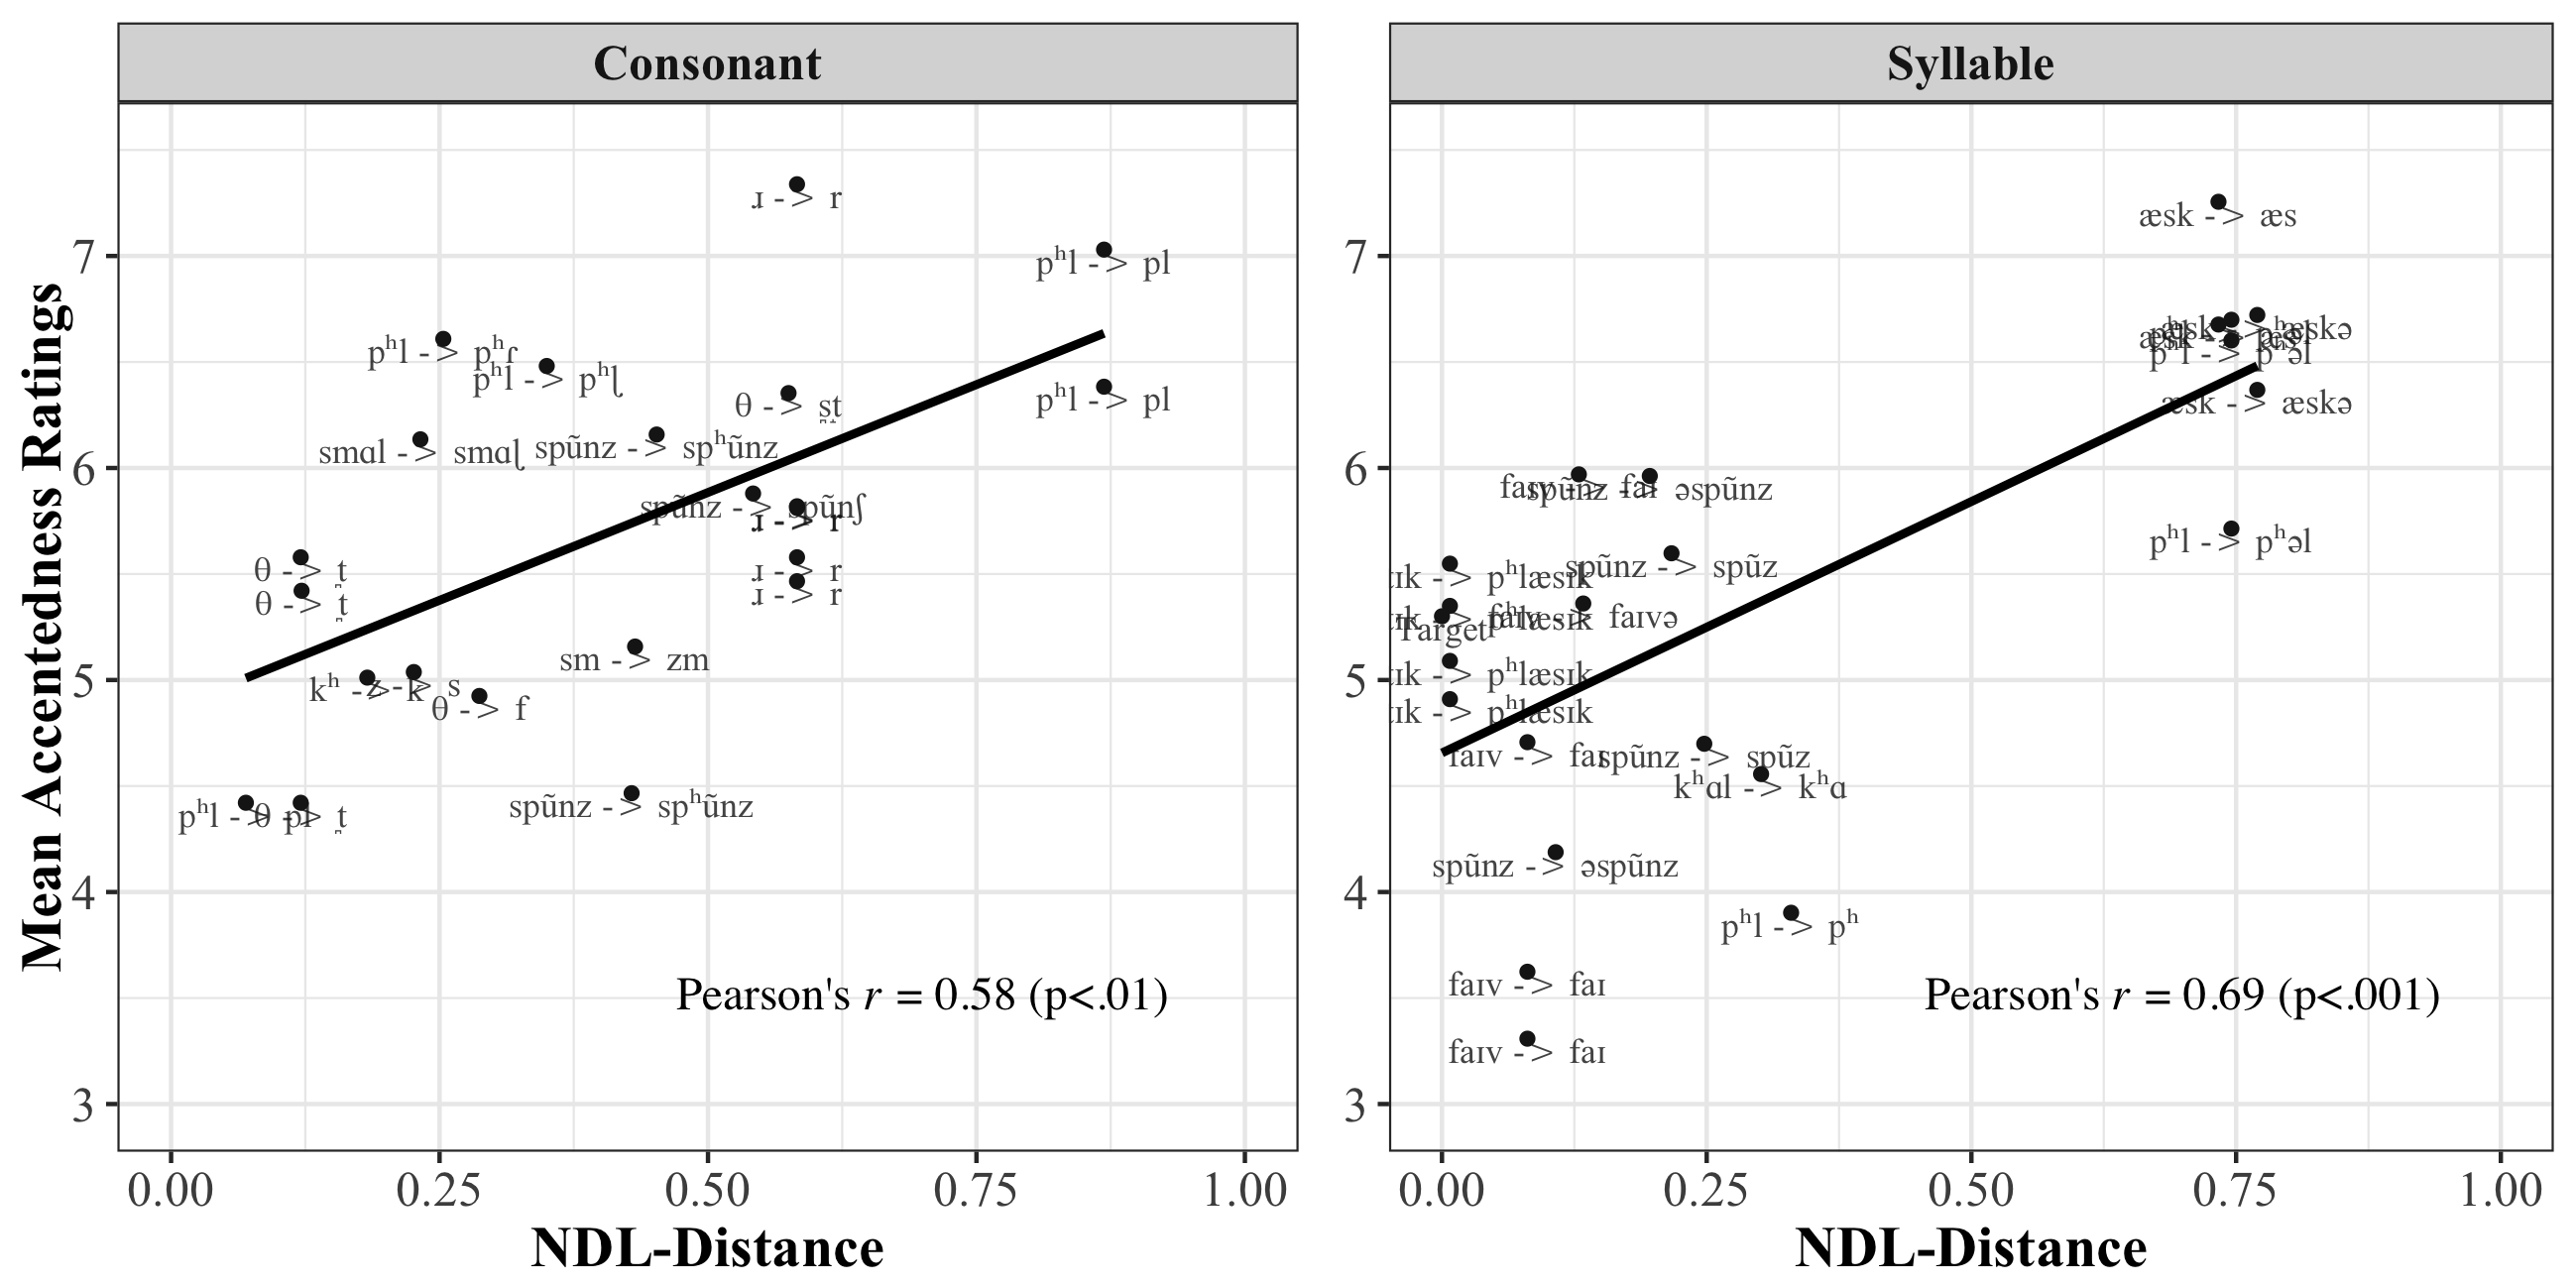
\includegraphics[width=1\textwidth]{figures/ndl/con_syl.png}
    \caption{Relationship between Accentedness and NDL-Distance (Consonant)}
    \label{fig:con}
  \figSpace
\end{figure}

Figure \ref{fig:con} shows that the mean accentedness ratings of different types of consonant mismatches positively correlates with NDL-distances (Pearson’s r = 0.58, p<.01). For example, the two instances of VOT-shortening on consonant cluster /pl/ in the context of “\textit{please call}” had an NDL-distance as large as 0.886 and the two instances were judged as being relatively more accented. The instance for VOT-shortening on /pl/ in the context of “\textit{small plastic}” had an NDL-distance as small as 0.070, and it was judged as being less accented. 

\begin{figure}[!h]
  \figSpace
    \centering
    % Created by tikzDevice version 0.12.3 on 2019-11-25 15:43:46
% !TEX encoding = UTF-8 Unicode
\begin{tikzpicture}[x=1pt,y=1pt]
\definecolor{fillColor}{RGB}{255,255,255}
\path[use as bounding box,fill=fillColor,fill opacity=0.00] (0,0) rectangle (339.67,289.08);
\begin{scope}
\path[clip] (  0.00,  0.00) rectangle (339.67,289.08);
\definecolor{drawColor}{RGB}{255,255,255}
\definecolor{fillColor}{RGB}{255,255,255}

\path[draw=drawColor,line width= 0.6pt,line join=round,line cap=round,fill=fillColor] (  0.00,  0.00) rectangle (339.67,289.08);
\end{scope}
\begin{scope}
\path[clip] ( 27.31, 30.69) rectangle (334.17,267.01);
\definecolor{fillColor}{RGB}{255,255,255}

\path[fill=fillColor] ( 27.31, 30.69) rectangle (334.17,267.01);
\definecolor{drawColor}{gray}{0.92}

\path[draw=drawColor,line width= 0.3pt,line join=round] ( 27.31, 65.30) --
	(334.17, 65.30);

\path[draw=drawColor,line width= 0.3pt,line join=round] ( 27.31,113.04) --
	(334.17,113.04);

\path[draw=drawColor,line width= 0.3pt,line join=round] ( 27.31,160.78) --
	(334.17,160.78);

\path[draw=drawColor,line width= 0.3pt,line join=round] ( 27.31,208.52) --
	(334.17,208.52);

\path[draw=drawColor,line width= 0.3pt,line join=round] ( 27.31,256.27) --
	(334.17,256.27);

\path[draw=drawColor,line width= 0.3pt,line join=round] ( 76.13, 30.69) --
	( 76.13,267.01);

\path[draw=drawColor,line width= 0.3pt,line join=round] (145.87, 30.69) --
	(145.87,267.01);

\path[draw=drawColor,line width= 0.3pt,line join=round] (215.61, 30.69) --
	(215.61,267.01);

\path[draw=drawColor,line width= 0.3pt,line join=round] (285.35, 30.69) --
	(285.35,267.01);

\path[draw=drawColor,line width= 0.6pt,line join=round] ( 27.31, 41.43) --
	(334.17, 41.43);

\path[draw=drawColor,line width= 0.6pt,line join=round] ( 27.31, 89.17) --
	(334.17, 89.17);

\path[draw=drawColor,line width= 0.6pt,line join=round] ( 27.31,136.91) --
	(334.17,136.91);

\path[draw=drawColor,line width= 0.6pt,line join=round] ( 27.31,184.65) --
	(334.17,184.65);

\path[draw=drawColor,line width= 0.6pt,line join=round] ( 27.31,232.40) --
	(334.17,232.40);

\path[draw=drawColor,line width= 0.6pt,line join=round] ( 41.26, 30.69) --
	( 41.26,267.01);

\path[draw=drawColor,line width= 0.6pt,line join=round] (111.00, 30.69) --
	(111.00,267.01);

\path[draw=drawColor,line width= 0.6pt,line join=round] (180.74, 30.69) --
	(180.74,267.01);

\path[draw=drawColor,line width= 0.6pt,line join=round] (250.48, 30.69) --
	(250.48,267.01);

\path[draw=drawColor,line width= 0.6pt,line join=round] (320.22, 30.69) --
	(320.22,267.01);
\definecolor{fillColor}{gray}{0.10}

\path[fill=fillColor] (101.73,165.45) circle (  1.96);

\path[fill=fillColor] (125.33,115.73) circle (  1.96);

\path[fill=fillColor] (245.83,216.96) circle (  1.96);

\path[fill=fillColor] ( 43.35,163.12) circle (  1.96);

\path[fill=fillColor] (249.24,171.01) circle (  1.96);

\path[fill=fillColor] (133.24, 84.50) circle (  1.96);

\path[fill=fillColor] (249.24,218.04) circle (  1.96);

\path[fill=fillColor] ( 78.48,154.14) circle (  1.96);

\path[fill=fillColor] (256.06,219.11) circle (  1.96);

\path[fill=fillColor] (110.36,122.55) circle (  1.96);

\path[fill=fillColor] ( 43.35,132.60) circle (  1.96);

\path[fill=fillColor] ( 96.01,182.86) circle (  1.96);

\path[fill=fillColor] ( 71.21, 98.14) circle (  1.96);

\path[fill=fillColor] (245.83,244.60) circle (  1.96);

\path[fill=fillColor] ( 77.32,183.22) circle (  1.96);

\path[fill=fillColor] ( 43.35,141.22) circle (  1.96);

\path[fill=fillColor] ( 63.77, 71.22) circle (  1.96);

\path[fill=fillColor] (256.06,202.24) circle (  1.96);

\path[fill=fillColor] ( 43.35,153.60) circle (  1.96);

\path[fill=fillColor] (249.24,213.37) circle (  1.96);

\path[fill=fillColor] ( 63.77, 56.15) circle (  1.96);

\path[fill=fillColor] ( 63.77,122.91) circle (  1.96);
\definecolor{drawColor}{RGB}{26,26,26}

\node[text=drawColor,text opacity=0.80,anchor=base,inner sep=0pt, outer sep=0pt, scale=  0.85] at (101.73,159.57) {spũnz$\rightarrow$spuz};

\node[text=drawColor,text opacity=0.80,anchor=base,inner sep=0pt, outer sep=0pt, scale=  0.85] at (125.33,109.85) {kʰɑl$\rightarrow$kʰɑ };

\node[text=drawColor,text opacity=0.80,anchor=base,inner sep=0pt, outer sep=0pt, scale=  0.85] at (245.83,211.08) {æsk$\rightarrow$æs};

\node[text=drawColor,text opacity=0.80,anchor=base,inner sep=0pt, outer sep=0pt, scale=  0.85] at ( 43.35,157.24) {pʰlæstɪk$\rightarrow$pʰlæsik};

\node[text=drawColor,text opacity=0.80,anchor=base,inner sep=0pt, outer sep=0pt, scale=  0.85] at (249.24,165.13) {pʰl$\rightarrow$pʰəl};

\node[text=drawColor,text opacity=0.80,anchor=base,inner sep=0pt, outer sep=0pt, scale=  0.85] at (133.24, 78.62) {pʰl$\rightarrow$pʰ};

\node[text=drawColor,text opacity=0.80,anchor=base,inner sep=0pt, outer sep=0pt, scale=  0.85] at (249.24,212.16) {pʰl$\rightarrow$pʰəl};

\node[text=drawColor,text opacity=0.80,anchor=base,inner sep=0pt, outer sep=0pt, scale=  0.85] at ( 78.48,148.26) {faɪv$\rightarrow$faɪvə};

\node[text=drawColor,text opacity=0.80,anchor=base,inner sep=0pt, outer sep=0pt, scale=  0.85] at (256.06,213.24) {æsk$\rightarrow$æskə};

\node[text=drawColor,text opacity=0.80,anchor=base,inner sep=0pt, outer sep=0pt, scale=  0.85] at (110.36,116.67) {spũnz$\rightarrow$spũz};

\node[text=drawColor,text opacity=0.80,anchor=base,inner sep=0pt, outer sep=0pt, scale=  0.85] at ( 43.35,126.73) {pʰlæstɪk$\rightarrow$pʰlæsɪk};

\node[text=drawColor,text opacity=0.80,anchor=base,inner sep=0pt, outer sep=0pt, scale=  0.85] at ( 96.01,176.98) {spũnz$\rightarrow$əspũnz};

\node[text=drawColor,text opacity=0.80,anchor=base,inner sep=0pt, outer sep=0pt, scale=  0.85] at ( 71.21, 92.26) {spũnz$\rightarrow$əspũnz};

\node[text=drawColor,text opacity=0.80,anchor=base,inner sep=0pt, outer sep=0pt, scale=  0.85] at (245.83,238.72) {æsk$\rightarrow$æs};

\node[text=drawColor,text opacity=0.80,anchor=base,inner sep=0pt, outer sep=0pt, scale=  0.85] at ( 77.32,177.34) {faɪv$\rightarrow$faɪ};

\node[text=drawColor,text opacity=0.80,anchor=base,inner sep=0pt, outer sep=0pt, scale=  0.85] at ( 43.35,135.34) {pʰlæstɪk$\rightarrow$plasik};

\node[text=drawColor,text opacity=0.80,anchor=base,inner sep=0pt, outer sep=0pt, scale=  0.85] at ( 63.77, 65.34) {faɪv$\rightarrow$faɪ};

\node[text=drawColor,text opacity=0.80,anchor=base,inner sep=0pt, outer sep=0pt, scale=  0.85] at (256.06,196.36) {æsk$\rightarrow$æskə};

\node[text=drawColor,text opacity=0.80,anchor=base,inner sep=0pt, outer sep=0pt, scale=  0.85] at ( 43.35,147.72) {pʰlæstɪk$\rightarrow$pʰlæsɪk};

\node[text=drawColor,text opacity=0.80,anchor=base,inner sep=0pt, outer sep=0pt, scale=  0.85] at (249.24,207.49) {pʰl$\rightarrow$pʰəl};

\node[text=drawColor,text opacity=0.80,anchor=base,inner sep=0pt, outer sep=0pt, scale=  0.85] at ( 63.77, 50.27) {faɪv$\rightarrow$faɪ};

\node[text=drawColor,text opacity=0.80,anchor=base,inner sep=0pt, outer sep=0pt, scale=  0.85] at ( 63.77,117.03) {faɪv$\rightarrow$faɪ};
\definecolor{drawColor}{RGB}{0,0,0}

\path[draw=drawColor,line width= 1.1pt,line join=round] ( 43.35,118.35) --
	( 46.04,119.49) --
	( 48.73,120.63) --
	( 51.43,121.77) --
	( 54.12,122.91) --
	( 56.81,124.05) --
	( 59.50,125.20) --
	( 62.20,126.34) --
	( 64.89,127.48) --
	( 67.58,128.62) --
	( 70.27,129.76) --
	( 72.97,130.90) --
	( 75.66,132.04) --
	( 78.35,133.18) --
	( 81.04,134.32) --
	( 83.74,135.47) --
	( 86.43,136.61) --
	( 89.12,137.75) --
	( 91.81,138.89) --
	( 94.51,140.03) --
	( 97.20,141.17) --
	( 99.89,142.31) --
	(102.58,143.45) --
	(105.28,144.60) --
	(107.97,145.74) --
	(110.66,146.88) --
	(113.35,148.02) --
	(116.05,149.16) --
	(118.74,150.30) --
	(121.43,151.44) --
	(124.12,152.58) --
	(126.82,153.72) --
	(129.51,154.87) --
	(132.20,156.01) --
	(134.89,157.15) --
	(137.59,158.29) --
	(140.28,159.43) --
	(142.97,160.57) --
	(145.67,161.71) --
	(148.36,162.85) --
	(151.05,164.00) --
	(153.74,165.14) --
	(156.44,166.28) --
	(159.13,167.42) --
	(161.82,168.56) --
	(164.51,169.70) --
	(167.21,170.84) --
	(169.90,171.98) --
	(172.59,173.13) --
	(175.28,174.27) --
	(177.98,175.41) --
	(180.67,176.55) --
	(183.36,177.69) --
	(186.05,178.83) --
	(188.75,179.97) --
	(191.44,181.11) --
	(194.13,182.25) --
	(196.82,183.40) --
	(199.52,184.54) --
	(202.21,185.68) --
	(204.90,186.82) --
	(207.59,187.96) --
	(210.29,189.10) --
	(212.98,190.24) --
	(215.67,191.38) --
	(218.36,192.53) --
	(221.06,193.67) --
	(223.75,194.81) --
	(226.44,195.95) --
	(229.13,197.09) --
	(231.83,198.23) --
	(234.52,199.37) --
	(237.21,200.51) --
	(239.90,201.65) --
	(242.60,202.80) --
	(245.29,203.94) --
	(247.98,205.08) --
	(250.68,206.22) --
	(253.37,207.36) --
	(256.06,208.50);

\node[text=drawColor,anchor=base west,inner sep=0pt, outer sep=0pt, scale=  1.14] at (162.89, 62.45) {Pearson's};

\node[text=drawColor,anchor=base west,inner sep=0pt, outer sep=0pt, scale=  1.14] at (214.67, 62.45) {\itshape  r};

\node[text=drawColor,anchor=base west,inner sep=0pt, outer sep=0pt, scale=  1.14] at (224.27, 62.45) { = 0.69 (p<.001)};
\definecolor{drawColor}{gray}{0.20}

\path[draw=drawColor,line width= 0.6pt,line join=round,line cap=round] ( 27.31, 30.69) rectangle (334.17,267.01);
\end{scope}
\begin{scope}
\path[clip] ( 27.31,267.01) rectangle (334.17,283.58);
\definecolor{drawColor}{gray}{0.20}
\definecolor{fillColor}{gray}{0.85}

\path[draw=drawColor,line width= 0.6pt,line join=round,line cap=round,fill=fillColor] ( 27.31,267.01) rectangle (334.17,283.58);
\definecolor{drawColor}{gray}{0.10}

\node[text=drawColor,anchor=base,inner sep=0pt, outer sep=0pt, scale=  0.88] at (180.74,272.26) {Syllable};
\end{scope}
\begin{scope}
\path[clip] (  0.00,  0.00) rectangle (339.67,289.08);
\definecolor{drawColor}{gray}{0.20}

\path[draw=drawColor,line width= 0.6pt,line join=round] ( 41.26, 27.94) --
	( 41.26, 30.69);

\path[draw=drawColor,line width= 0.6pt,line join=round] (111.00, 27.94) --
	(111.00, 30.69);

\path[draw=drawColor,line width= 0.6pt,line join=round] (180.74, 27.94) --
	(180.74, 30.69);

\path[draw=drawColor,line width= 0.6pt,line join=round] (250.48, 27.94) --
	(250.48, 30.69);

\path[draw=drawColor,line width= 0.6pt,line join=round] (320.22, 27.94) --
	(320.22, 30.69);
\end{scope}
\begin{scope}
\path[clip] (  0.00,  0.00) rectangle (339.67,289.08);
\definecolor{drawColor}{gray}{0.30}

\node[text=drawColor,anchor=base,inner sep=0pt, outer sep=0pt, scale=  0.88] at ( 41.26, 19.68) {0.00};

\node[text=drawColor,anchor=base,inner sep=0pt, outer sep=0pt, scale=  0.88] at (111.00, 19.68) {0.25};

\node[text=drawColor,anchor=base,inner sep=0pt, outer sep=0pt, scale=  0.88] at (180.74, 19.68) {0.50};

\node[text=drawColor,anchor=base,inner sep=0pt, outer sep=0pt, scale=  0.88] at (250.48, 19.68) {0.75};

\node[text=drawColor,anchor=base,inner sep=0pt, outer sep=0pt, scale=  0.88] at (320.22, 19.68) {1.00};
\end{scope}
\begin{scope}
\path[clip] (  0.00,  0.00) rectangle (339.67,289.08);
\definecolor{drawColor}{gray}{0.30}

\node[text=drawColor,anchor=base east,inner sep=0pt, outer sep=0pt, scale=  0.88] at ( 22.36, 38.40) {3};

\node[text=drawColor,anchor=base east,inner sep=0pt, outer sep=0pt, scale=  0.88] at ( 22.36, 86.14) {4};

\node[text=drawColor,anchor=base east,inner sep=0pt, outer sep=0pt, scale=  0.88] at ( 22.36,133.88) {5};

\node[text=drawColor,anchor=base east,inner sep=0pt, outer sep=0pt, scale=  0.88] at ( 22.36,181.62) {6};

\node[text=drawColor,anchor=base east,inner sep=0pt, outer sep=0pt, scale=  0.88] at ( 22.36,229.37) {7};
\end{scope}
\begin{scope}
\path[clip] (  0.00,  0.00) rectangle (339.67,289.08);
\definecolor{drawColor}{gray}{0.20}

\path[draw=drawColor,line width= 0.6pt,line join=round] ( 24.56, 41.43) --
	( 27.31, 41.43);

\path[draw=drawColor,line width= 0.6pt,line join=round] ( 24.56, 89.17) --
	( 27.31, 89.17);

\path[draw=drawColor,line width= 0.6pt,line join=round] ( 24.56,136.91) --
	( 27.31,136.91);

\path[draw=drawColor,line width= 0.6pt,line join=round] ( 24.56,184.65) --
	( 27.31,184.65);

\path[draw=drawColor,line width= 0.6pt,line join=round] ( 24.56,232.40) --
	( 27.31,232.40);
\end{scope}
\begin{scope}
\path[clip] (  0.00,  0.00) rectangle (339.67,289.08);
\definecolor{drawColor}{RGB}{0,0,0}

\node[text=drawColor,anchor=base,inner sep=0pt, outer sep=0pt, scale=  1.10] at (180.74,  7.64) {NDL-Distance};
\end{scope}
\begin{scope}
\path[clip] (  0.00,  0.00) rectangle (339.67,289.08);
\definecolor{drawColor}{RGB}{0,0,0}

\node[text=drawColor,rotate= 90.00,anchor=base,inner sep=0pt, outer sep=0pt, scale=  1.10] at ( 13.08,148.85) {Mean Accentedness Ratings};
\end{scope}
\end{tikzpicture}

  %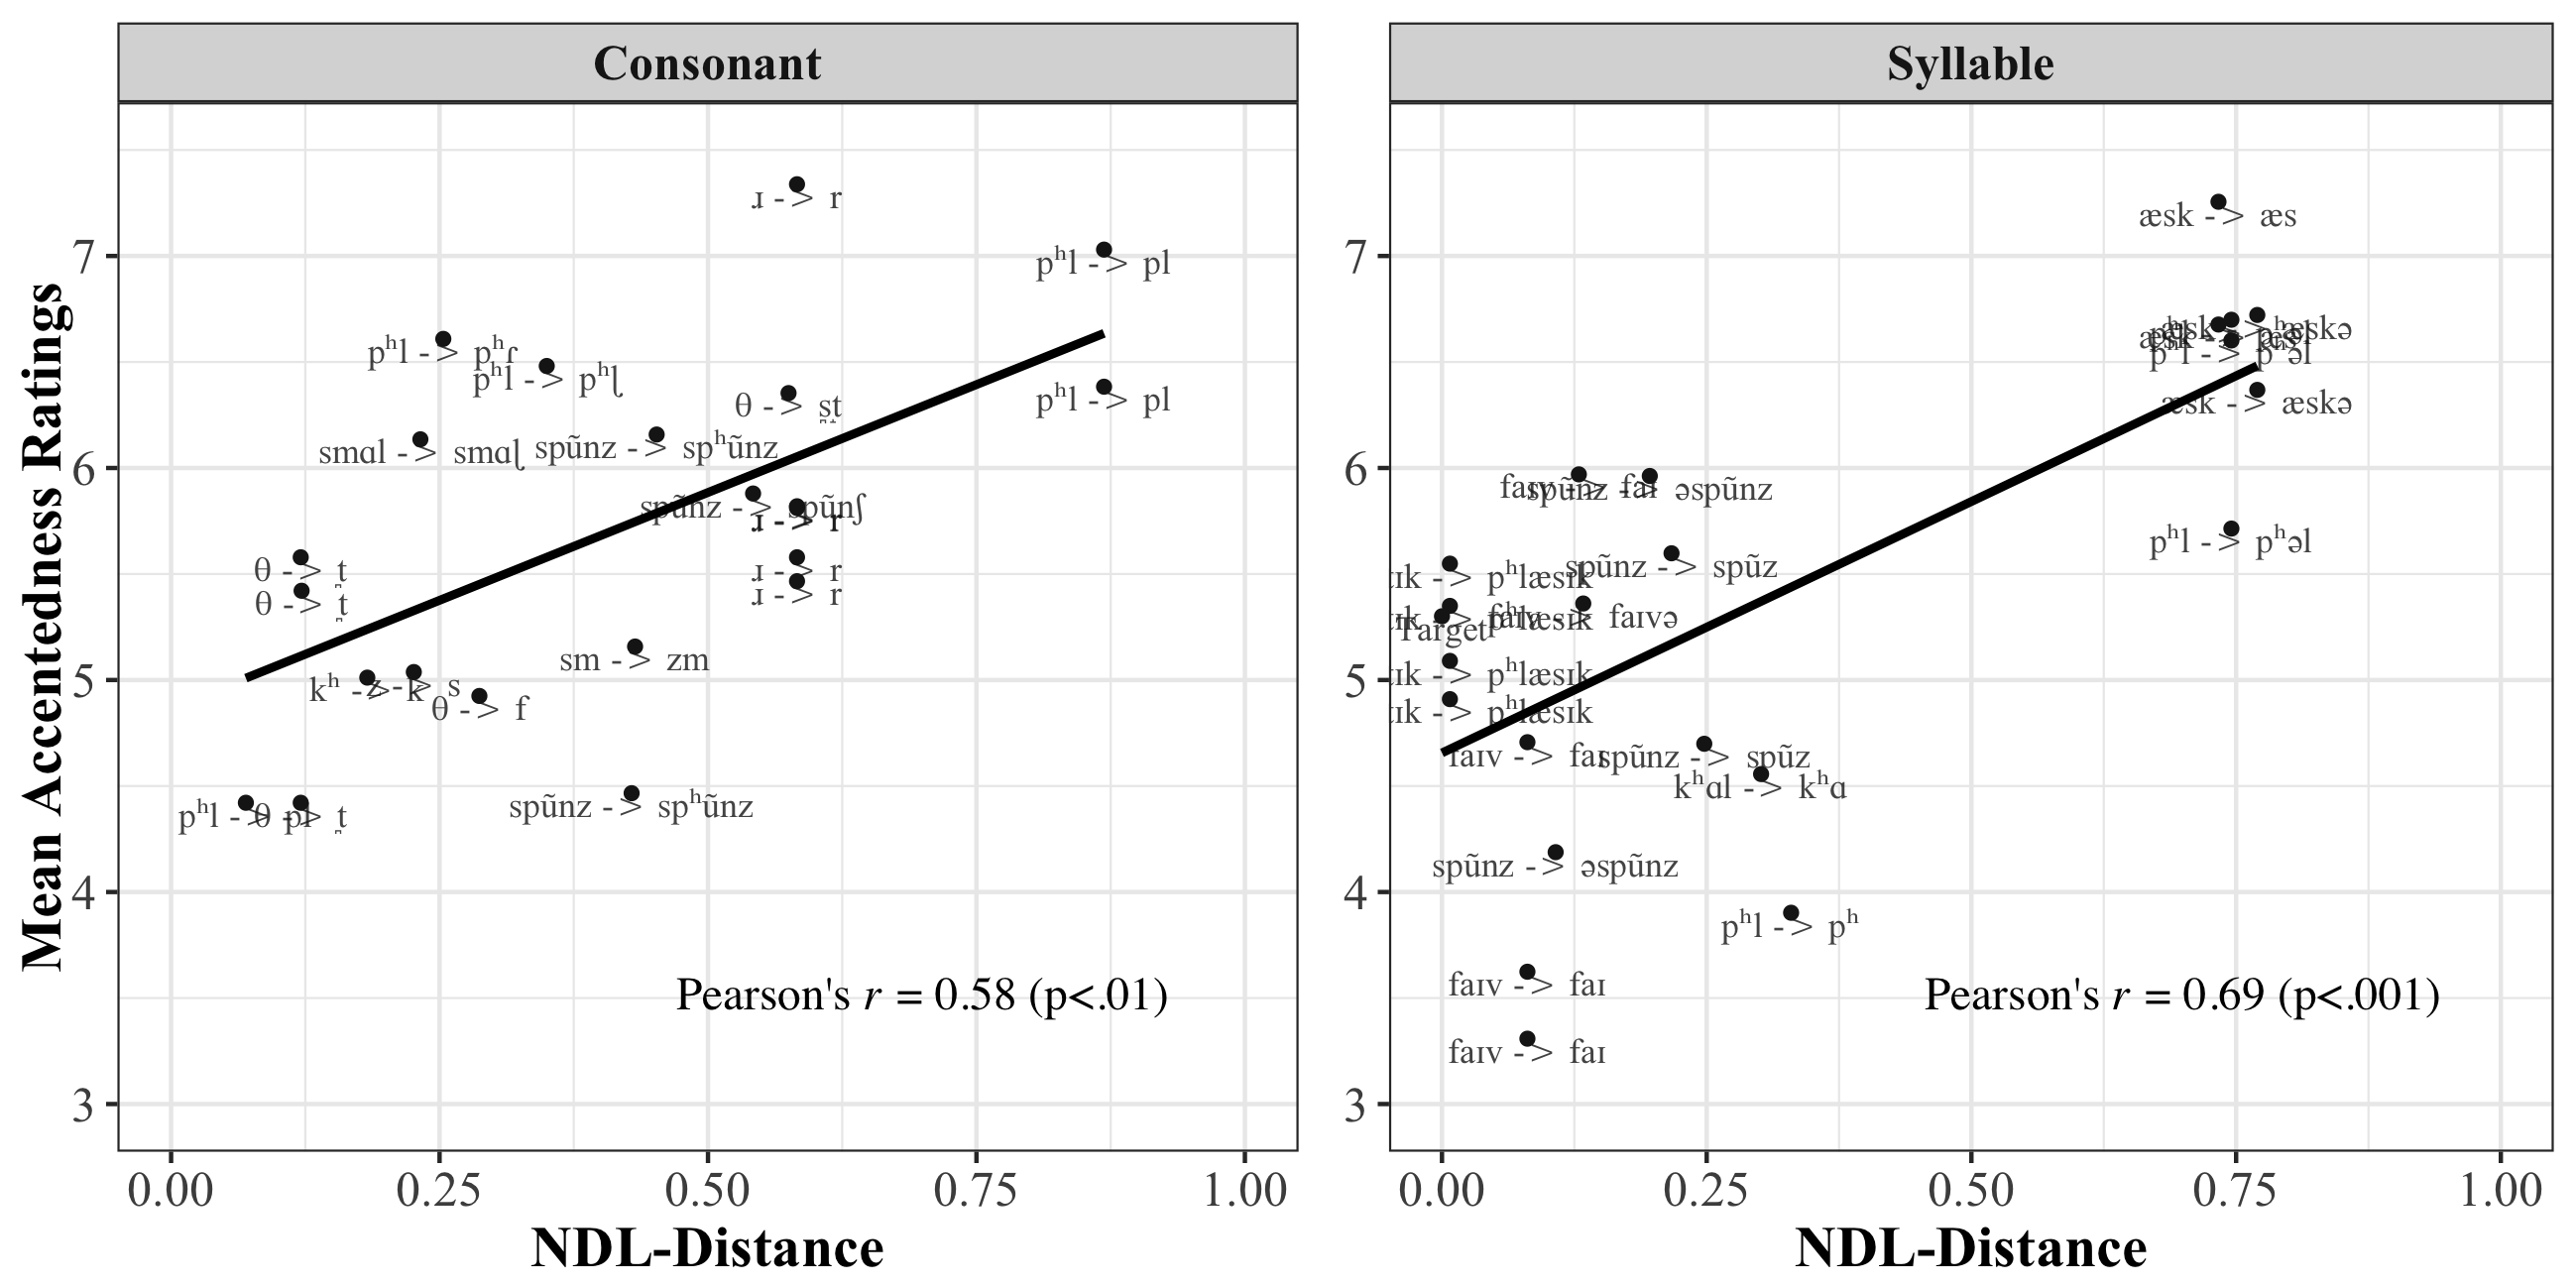
\includegraphics[width=1\textwidth]{figures/ndl/con_syl.png}
    \caption{Relationship between Accentedness and NDL-Distance (Syllable)}
    \label{fig:syl}
  \figSpace
\end{figure}

There are, however, a few discrepancies. The NDL-distance failed to model accentedness for stimuli with non-English phonemes. For example, one of the four cases for /ɹ/-trilling (i.e. /ɹ/ $\rightarrow$/r/) was assigned a relatively higher accentedness rating, but its NDL-distance was not as large as expected. The use of the retroflex [ɭ] such as [smɑl]$\rightarrow$[smɑɭ] was also rated as very accented. Possible reasons for the discrepancies are discussed in the Discussion section of this chapter. However, NDL-distances for these stimuli were smaller than expected. NDL-distances did correlate well with accentedness ratings of stimuli with consonant mismatches. 

Figure \ref{fig:syl} shows the relationship between NDL-distances and ratings of stimuli with syllable mismatches. There is also a clear positive correlation between NDL-distances and accentedness ratings of stimuli with syllable mismatches (Pearson’s r = 0.69, p<.001). For example, the NDL-distances for stimuli with vowel epenthesis are around 0.750, while the NDL-distances for stimuli with segment deletion are generally lower than 0.500. Accentedness ratings show that vowel epenthesis was indeed judged as being more accented than segment deletion. Interestingly, /k/-deletion in the context of “\textit{ask her}” was rated as relatively more accented than other types of consonant deletion. This particular exception is also captured by the NDL-distance measurement. 

The correlation between NDL-distances and accentedness ratings of vowel mismatches is also positive (Pearson’s r = 0.44, p<.05). Figure \ref{fig:vow} illustrates the relationship between NDL-distances and mean accentedness ratings of stimuli with vowel mismatches. 

\begin{figure}[!h]
  \figSpace
    \centering
        % Created by tikzDevice version 0.12.3 on 2019-11-25 15:56:25
% !TEX encoding = UTF-8 Unicode
\begin{tikzpicture}[x=1pt,y=1pt]
\definecolor{fillColor}{RGB}{255,255,255}
\path[use as bounding box,fill=fillColor,fill opacity=0.00] (0,0) rectangle (325.21,289.08);
\begin{scope}
\path[clip] (  0.00,  0.00) rectangle (325.21,289.08);
\definecolor{drawColor}{RGB}{255,255,255}
\definecolor{fillColor}{RGB}{255,255,255}

\path[draw=drawColor,line width= 0.6pt,line join=round,line cap=round,fill=fillColor] (  0.00,  0.00) rectangle (325.21,289.08);
\end{scope}
\begin{scope}
\path[clip] ( 27.31, 30.69) rectangle (319.71,283.58);
\definecolor{fillColor}{RGB}{255,255,255}

\path[fill=fillColor] ( 27.31, 30.69) rectangle (319.71,283.58);
\definecolor{drawColor}{gray}{0.92}

\path[draw=drawColor,line width= 0.3pt,line join=round] ( 27.31, 67.73) --
	(319.71, 67.73);

\path[draw=drawColor,line width= 0.3pt,line join=round] ( 27.31,118.82) --
	(319.71,118.82);

\path[draw=drawColor,line width= 0.3pt,line join=round] ( 27.31,169.91) --
	(319.71,169.91);

\path[draw=drawColor,line width= 0.3pt,line join=round] ( 27.31,221.00) --
	(319.71,221.00);

\path[draw=drawColor,line width= 0.3pt,line join=round] ( 27.31,272.08) --
	(319.71,272.08);

\path[draw=drawColor,line width= 0.3pt,line join=round] ( 73.83, 30.69) --
	( 73.83,283.58);

\path[draw=drawColor,line width= 0.3pt,line join=round] (140.29, 30.69) --
	(140.29,283.58);

\path[draw=drawColor,line width= 0.3pt,line join=round] (206.74, 30.69) --
	(206.74,283.58);

\path[draw=drawColor,line width= 0.3pt,line join=round] (273.20, 30.69) --
	(273.20,283.58);

\path[draw=drawColor,line width= 0.6pt,line join=round] ( 27.31, 42.18) --
	(319.71, 42.18);

\path[draw=drawColor,line width= 0.6pt,line join=round] ( 27.31, 93.27) --
	(319.71, 93.27);

\path[draw=drawColor,line width= 0.6pt,line join=round] ( 27.31,144.36) --
	(319.71,144.36);

\path[draw=drawColor,line width= 0.6pt,line join=round] ( 27.31,195.45) --
	(319.71,195.45);

\path[draw=drawColor,line width= 0.6pt,line join=round] ( 27.31,246.54) --
	(319.71,246.54);

\path[draw=drawColor,line width= 0.6pt,line join=round] ( 40.60, 30.69) --
	( 40.60,283.58);

\path[draw=drawColor,line width= 0.6pt,line join=round] (107.06, 30.69) --
	(107.06,283.58);

\path[draw=drawColor,line width= 0.6pt,line join=round] (173.51, 30.69) --
	(173.51,283.58);

\path[draw=drawColor,line width= 0.6pt,line join=round] (239.97, 30.69) --
	(239.97,283.58);

\path[draw=drawColor,line width= 0.6pt,line join=round] (306.42, 30.69) --
	(306.42,283.58);
\definecolor{fillColor}{gray}{0.10}

\path[fill=fillColor] (124.09,175.86) circle (  1.96);

\path[fill=fillColor] ( 56.24, 90.97) circle (  1.96);

\path[fill=fillColor] ( 63.39,190.07) circle (  1.96);

\path[fill=fillColor] ( 40.60,116.70) circle (  1.96);

\path[fill=fillColor] ( 85.89,135.53) circle (  1.96);

\path[fill=fillColor] ( 84.35,136.29) circle (  1.96);

\path[fill=fillColor] ( 91.03,105.56) circle (  1.96);

\path[fill=fillColor] ( 84.35,163.57) circle (  1.96);

\path[fill=fillColor] ( 76.64,124.00) circle (  1.96);

\path[fill=fillColor] (159.45,122.08) circle (  1.96);

\path[fill=fillColor] (123.16,142.44) circle (  1.96);

\path[fill=fillColor] (159.38,166.64) circle (  1.96);

\path[fill=fillColor] ( 40.60, 92.50) circle (  1.96);

\path[fill=fillColor] (162.44,196.99) circle (  1.96);

\path[fill=fillColor] (100.41,187.00) circle (  1.96);

\path[fill=fillColor] (108.39,169.33) circle (  1.96);

\path[fill=fillColor] (100.41,139.37) circle (  1.96);

\path[fill=fillColor] (100.41,172.40) circle (  1.96);

\path[fill=fillColor] (158.89,201.21) circle (  1.96);

\path[fill=fillColor] (173.51,134.57) circle (  1.96);

\path[fill=fillColor] ( 84.35,183.93) circle (  1.96);

\path[fill=fillColor] (129.41, 81.75) circle (  1.96);

\path[fill=fillColor] ( 40.60, 77.14) circle (  1.96);

\path[fill=fillColor] (173.51,168.56) circle (  1.96);

\path[fill=fillColor] (136.15,146.67) circle (  1.96);
\definecolor{drawColor}{RGB}{26,26,26}

\node[text=drawColor,text opacity=0.80,anchor=base,inner sep=0pt, outer sep=0pt, scale=  0.85] at (124.09,169.98) {ɑ$\rightarrow$o};

\node[text=drawColor,text opacity=0.80,anchor=base,inner sep=0pt, outer sep=0pt, scale=  0.85] at ( 56.24, 85.09) {ũ$\rightarrow$ʊ};

\node[text=drawColor,text opacity=0.80,anchor=base,inner sep=0pt, outer sep=0pt, scale=  0.85] at ( 63.39,184.19) {æ$\rightarrow$a};

\node[text=drawColor,text opacity=0.80,anchor=base,inner sep=0pt, outer sep=0pt, scale=  0.85] at ( 40.60,110.82) {æ$\rightarrow$æ̞};

\node[text=drawColor,text opacity=0.80,anchor=base,inner sep=0pt, outer sep=0pt, scale=  0.85] at ( 85.89,129.65) {æ$\rightarrow$a};

\node[text=drawColor,text opacity=0.80,anchor=base,inner sep=0pt, outer sep=0pt, scale=  0.85] at ( 84.35,130.41) {æ$\rightarrow$a};

\node[text=drawColor,text opacity=0.80,anchor=base,inner sep=0pt, outer sep=0pt, scale=  0.85] at ( 91.03, 99.68) {ũ$\rightarrow$ũ̟};

\node[text=drawColor,text opacity=0.80,anchor=base,inner sep=0pt, outer sep=0pt, scale=  0.85] at ( 84.35,157.69) {æ$\rightarrow$a};

\node[text=drawColor,text opacity=0.80,anchor=base,inner sep=0pt, outer sep=0pt, scale=  0.85] at ( 76.64,118.12) {ɑ$\rightarrow$ɔ};

\node[text=drawColor,text opacity=0.80,anchor=base,inner sep=0pt, outer sep=0pt, scale=  0.85] at (159.45,116.20) {ɪ$\rightarrow$i};

\node[text=drawColor,text opacity=0.80,anchor=base,inner sep=0pt, outer sep=0pt, scale=  0.85] at (123.16,136.56) {ɪ$\rightarrow$i};

\node[text=drawColor,text opacity=0.80,anchor=base,inner sep=0pt, outer sep=0pt, scale=  0.85] at (159.38,160.76) {ɪ$\rightarrow$i};

\node[text=drawColor,text opacity=0.80,anchor=base,inner sep=0pt, outer sep=0pt, scale=  0.85] at ( 40.60, 86.62) {ɑ$\rightarrow$ɔ};

\node[text=drawColor,text opacity=0.80,anchor=base,inner sep=0pt, outer sep=0pt, scale=  0.85] at (162.44,191.11) {aɪ$\rightarrow$ɑɪ};

\node[text=drawColor,text opacity=0.80,anchor=base,inner sep=0pt, outer sep=0pt, scale=  0.85] at (100.41,181.12) {ɪ$\rightarrow$i};

\node[text=drawColor,text opacity=0.80,anchor=base,inner sep=0pt, outer sep=0pt, scale=  0.85] at (108.39,163.45) {æ$\rightarrow$æ̝};

\node[text=drawColor,text opacity=0.80,anchor=base,inner sep=0pt, outer sep=0pt, scale=  0.85] at (100.41,133.49) {ɪ$\rightarrow$i};

\node[text=drawColor,text opacity=0.80,anchor=base,inner sep=0pt, outer sep=0pt, scale=  0.85] at (100.41,166.52) {ɪ$\rightarrow$i};

\node[text=drawColor,text opacity=0.80,anchor=base,inner sep=0pt, outer sep=0pt, scale=  0.85] at (158.89,195.33) {aɪ$\rightarrow$a};

\node[text=drawColor,text opacity=0.80,anchor=base,inner sep=0pt, outer sep=0pt, scale=  0.85] at (173.51,128.69) {ɑ$\rightarrow$o};

\node[text=drawColor,text opacity=0.80,anchor=base,inner sep=0pt, outer sep=0pt, scale=  0.85] at ( 84.35,178.05) {æ$\rightarrow$ɑ};

\node[text=drawColor,text opacity=0.80,anchor=base,inner sep=0pt, outer sep=0pt, scale=  0.85] at (129.41, 75.87) {ɪ$\rightarrow$i};

\node[text=drawColor,text opacity=0.80,anchor=base,inner sep=0pt, outer sep=0pt, scale=  0.85] at ( 40.60, 71.26) {ɑ$\rightarrow$ɔ};

\node[text=drawColor,text opacity=0.80,anchor=base,inner sep=0pt, outer sep=0pt, scale=  0.85] at (173.51,162.68) {ɑ$\rightarrow$o};

\node[text=drawColor,text opacity=0.80,anchor=base,inner sep=0pt, outer sep=0pt, scale=  0.85] at (136.15,140.79) {ɪ$\rightarrow$i};
\definecolor{drawColor}{RGB}{0,0,0}

\path[draw=drawColor,line width= 1.1pt,line join=round] ( 40.60,119.88) --
	( 42.29,120.52) --
	( 43.97,121.16) --
	( 45.65,121.79) --
	( 47.33,122.43) --
	( 49.02,123.07) --
	( 50.70,123.71) --
	( 52.38,124.35) --
	( 54.06,124.99) --
	( 55.75,125.63) --
	( 57.43,126.27) --
	( 59.11,126.91) --
	( 60.79,127.55) --
	( 62.48,128.19) --
	( 64.16,128.83) --
	( 65.84,129.47) --
	( 67.52,130.11) --
	( 69.21,130.75) --
	( 70.89,131.38) --
	( 72.57,132.02) --
	( 74.25,132.66) --
	( 75.93,133.30) --
	( 77.62,133.94) --
	( 79.30,134.58) --
	( 80.98,135.22) --
	( 82.66,135.86) --
	( 84.35,136.50) --
	( 86.03,137.14) --
	( 87.71,137.78) --
	( 89.39,138.42) --
	( 91.08,139.06) --
	( 92.76,139.70) --
	( 94.44,140.34) --
	( 96.12,140.97) --
	( 97.81,141.61) --
	( 99.49,142.25) --
	(101.17,142.89) --
	(102.85,143.53) --
	(104.54,144.17) --
	(106.22,144.81) --
	(107.90,145.45) --
	(109.58,146.09) --
	(111.27,146.73) --
	(112.95,147.37) --
	(114.63,148.01) --
	(116.31,148.65) --
	(117.99,149.29) --
	(119.68,149.93) --
	(121.36,150.56) --
	(123.04,151.20) --
	(124.72,151.84) --
	(126.41,152.48) --
	(128.09,153.12) --
	(129.77,153.76) --
	(131.45,154.40) --
	(133.14,155.04) --
	(134.82,155.68) --
	(136.50,156.32) --
	(138.18,156.96) --
	(139.87,157.60) --
	(141.55,158.24) --
	(143.23,158.88) --
	(144.91,159.52) --
	(146.60,160.15) --
	(148.28,160.79) --
	(149.96,161.43) --
	(151.64,162.07) --
	(153.33,162.71) --
	(155.01,163.35) --
	(156.69,163.99) --
	(158.37,164.63) --
	(160.05,165.27) --
	(161.74,165.91) --
	(163.42,166.55) --
	(165.10,167.19) --
	(166.78,167.83) --
	(168.47,168.47) --
	(170.15,169.11) --
	(171.83,169.74) --
	(173.51,170.38);

\node[text=drawColor,anchor=base west,inner sep=0pt, outer sep=0pt, scale=  1.14] at (182.46, 64.88) {Pearson's};

\node[text=drawColor,anchor=base west,inner sep=0pt, outer sep=0pt, scale=  1.14] at (234.24, 64.88) {\itshape  r};

\node[text=drawColor,anchor=base west,inner sep=0pt, outer sep=0pt, scale=  1.14] at (243.84, 64.88) {  = 0.44 (p<.05)};
\definecolor{drawColor}{gray}{0.20}

\path[draw=drawColor,line width= 0.6pt,line join=round,line cap=round] ( 27.31, 30.69) rectangle (319.71,283.58);
\end{scope}
\begin{scope}
\path[clip] (  0.00,  0.00) rectangle (325.21,289.08);
\definecolor{drawColor}{gray}{0.30}

\node[text=drawColor,anchor=base east,inner sep=0pt, outer sep=0pt, scale=  0.88] at ( 22.36, 39.15) {3};

\node[text=drawColor,anchor=base east,inner sep=0pt, outer sep=0pt, scale=  0.88] at ( 22.36, 90.24) {4};

\node[text=drawColor,anchor=base east,inner sep=0pt, outer sep=0pt, scale=  0.88] at ( 22.36,141.33) {5};

\node[text=drawColor,anchor=base east,inner sep=0pt, outer sep=0pt, scale=  0.88] at ( 22.36,192.42) {6};

\node[text=drawColor,anchor=base east,inner sep=0pt, outer sep=0pt, scale=  0.88] at ( 22.36,243.51) {7};
\end{scope}
\begin{scope}
\path[clip] (  0.00,  0.00) rectangle (325.21,289.08);
\definecolor{drawColor}{gray}{0.20}

\path[draw=drawColor,line width= 0.6pt,line join=round] ( 24.56, 42.18) --
	( 27.31, 42.18);

\path[draw=drawColor,line width= 0.6pt,line join=round] ( 24.56, 93.27) --
	( 27.31, 93.27);

\path[draw=drawColor,line width= 0.6pt,line join=round] ( 24.56,144.36) --
	( 27.31,144.36);

\path[draw=drawColor,line width= 0.6pt,line join=round] ( 24.56,195.45) --
	( 27.31,195.45);

\path[draw=drawColor,line width= 0.6pt,line join=round] ( 24.56,246.54) --
	( 27.31,246.54);
\end{scope}
\begin{scope}
\path[clip] (  0.00,  0.00) rectangle (325.21,289.08);
\definecolor{drawColor}{gray}{0.20}

\path[draw=drawColor,line width= 0.6pt,line join=round] ( 40.60, 27.94) --
	( 40.60, 30.69);

\path[draw=drawColor,line width= 0.6pt,line join=round] (107.06, 27.94) --
	(107.06, 30.69);

\path[draw=drawColor,line width= 0.6pt,line join=round] (173.51, 27.94) --
	(173.51, 30.69);

\path[draw=drawColor,line width= 0.6pt,line join=round] (239.97, 27.94) --
	(239.97, 30.69);

\path[draw=drawColor,line width= 0.6pt,line join=round] (306.42, 27.94) --
	(306.42, 30.69);
\end{scope}
\begin{scope}
\path[clip] (  0.00,  0.00) rectangle (325.21,289.08);
\definecolor{drawColor}{gray}{0.30}

\node[text=drawColor,anchor=base,inner sep=0pt, outer sep=0pt, scale=  0.88] at ( 40.60, 19.68) {0.00};

\node[text=drawColor,anchor=base,inner sep=0pt, outer sep=0pt, scale=  0.88] at (107.06, 19.68) {0.25};

\node[text=drawColor,anchor=base,inner sep=0pt, outer sep=0pt, scale=  0.88] at (173.51, 19.68) {0.50};

\node[text=drawColor,anchor=base,inner sep=0pt, outer sep=0pt, scale=  0.88] at (239.97, 19.68) {0.75};

\node[text=drawColor,anchor=base,inner sep=0pt, outer sep=0pt, scale=  0.88] at (306.42, 19.68) {1.00};
\end{scope}
\begin{scope}
\path[clip] (  0.00,  0.00) rectangle (325.21,289.08);
\definecolor{drawColor}{RGB}{0,0,0}

\node[text=drawColor,anchor=base,inner sep=0pt, outer sep=0pt, scale=  1.10] at (173.51,  7.64) {NDL-Distance};
\end{scope}
\begin{scope}
\path[clip] (  0.00,  0.00) rectangle (325.21,289.08);
\definecolor{drawColor}{RGB}{0,0,0}

\node[text=drawColor,rotate= 90.00,anchor=base,inner sep=0pt, outer sep=0pt, scale=  1.10] at ( 13.08,157.13) {Mean Accentedness Ratings};
\end{scope}
\end{tikzpicture}

	%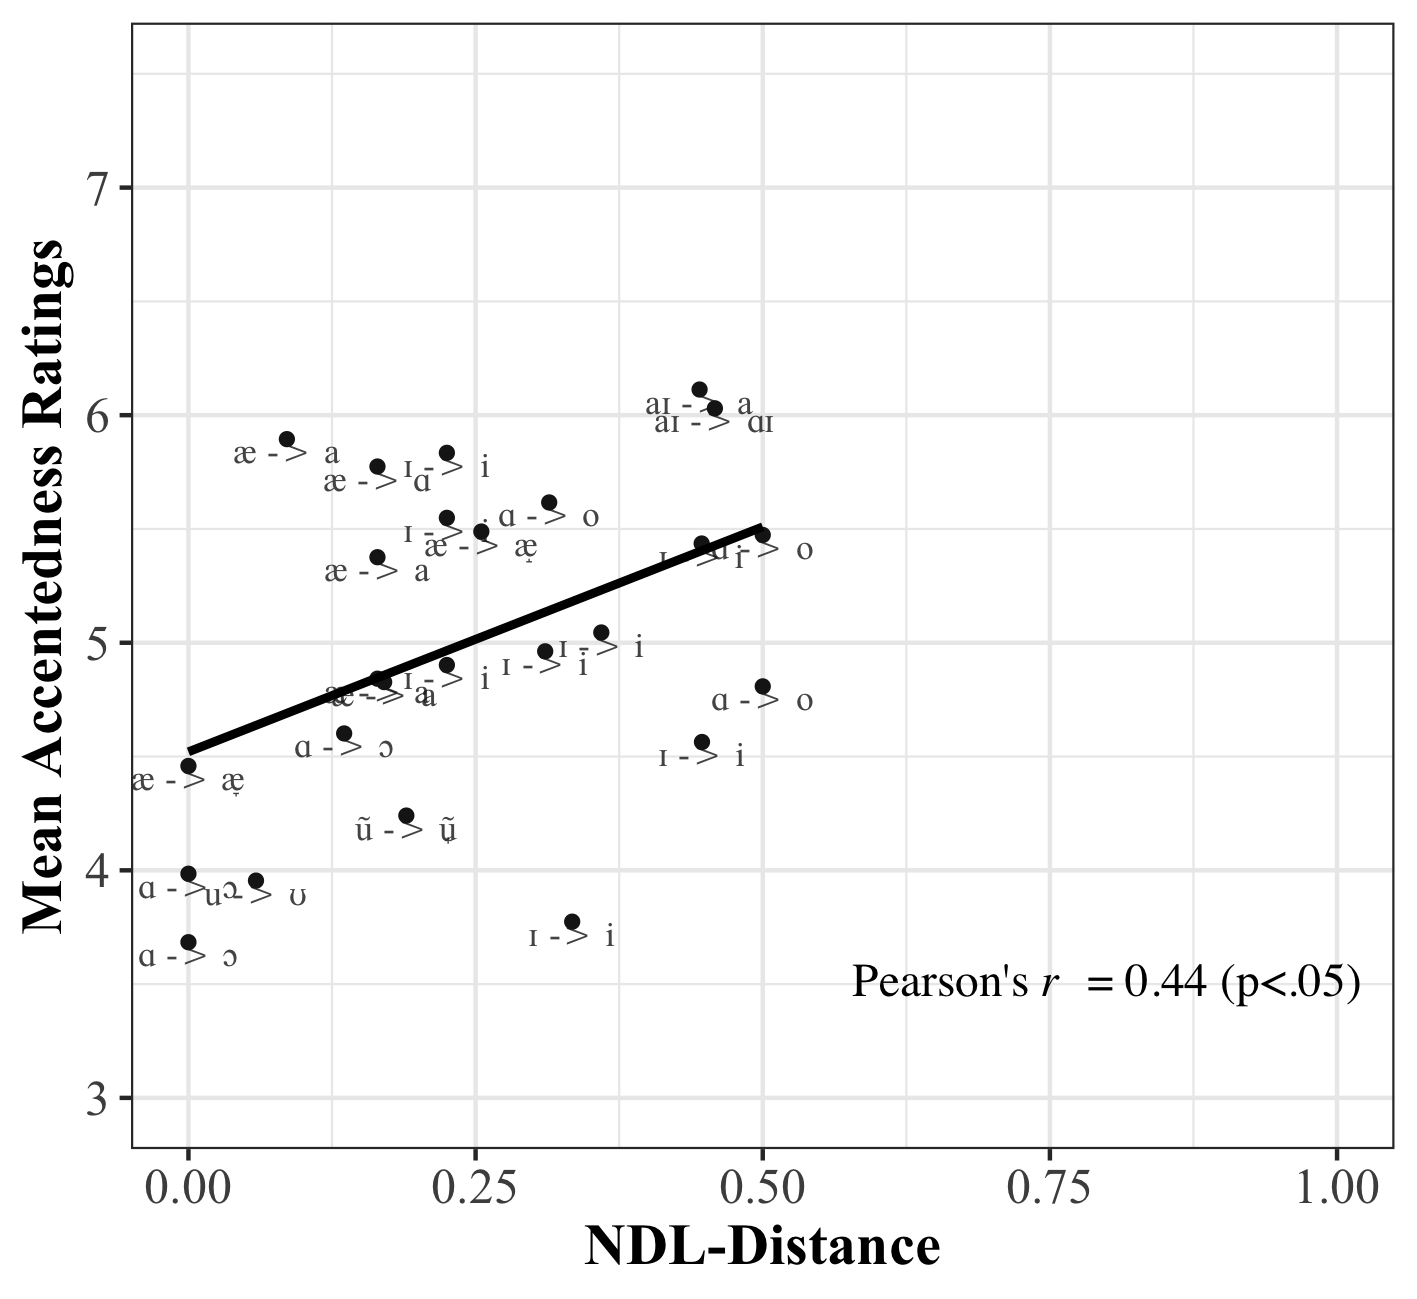
\includegraphics[width=0.75\textwidth]{figures/ndl/vow.png}
    \caption{Relationship between Accentedness and NDL-Distance (Vowel)}
    \label{fig:vow}
  \figSpace
\end{figure}

Dialectal variations such as [ɑ]$\rightarrow$[ɔ] in words “\textit{small}” and “call” were assigned smaller NDL-distances. Non-dialectal variations such [aɪ]$\rightarrow$[a] and [aɪ]$\rightarrow$[ɑɪ] in word “\textit{five}” were assigned relatively larger NDL-distances. Dialectal variations indeed received relatively lower ratings than did non-dialectal variations. Therefore, the NDL-distance explains rating differences between vowel mismatches to a certain degree. However, the range of NDL-distances for stimuli with vowel mismatches is restricted to the range from 0 to 0.500. It is known in the field of statistics that a restricted range severely affects correlation. Therefore, the Pearson correlation calculated above might not be meaningful. The reason for the restriction of NDL-distances (i.e., a narrower range) was because vowels of the L1 productions exhibit a relatively higher degree of variation, especially when diacritics are considered. The NDL algorithm therefore assigned lower association strength to trigram cues involving vowels. In other words, vowels in an utterance did not contribute as much to the association strength as did consonants, unless the vowels are epenthetic, which was considered an issue of syllable mismatch. As a result, the range of NDL-distances for vowel mismatches is limited to under 0.500. In order to fully examine the possible effect of NDL-distances on accentedness of vowel mismatches, a wider range of NDL-distance is required.

\subsection{Summary}

Results of Experiments 1 and 2 show that the frequency of occurrence of a speech pattern in L1 speech could potentially affect the accentedness judgment on the phonetic pattern. For example, pronouncing “\textit{thick}” as [tɪk] or [fɪk] was observed in L1 speech data. L2 stimuli involving pronouncing “\textit{thick}” as [tɪk] or [fɪk] were judged as less accented. On the other hand, pronouncing “\textit{ask}” as [æsk] was not observed in L1 speech data. [æskə] was indeed judged as relatively more accented. These results indicate that the raters were aware of which speech patterns are allowed in L1 speech and have made their accentedness judgment based on such knowledge.  Experiments 1 and 2 made a general claim that consonant mismatches are in general more accented than syllable or vowel mismatches. However, frequency of occurrence of a speech pattern in L1 speech could have potentially skewed the result. Experiment 3 described in the current chapter implements an NDL approach to account for the raters’ phonetic and phonological knowledge with regard to the five contexts. 

Experiment 3 constructed an L1 production model and subsequently measured the NDL-distance between L2 productions and their corresponding L1 productions. The calculation was based on the notion of association strength, which was defined as the probability that a trigram phonetic cue (e.g., \textit{\#æs}, \textit{æsk}, \textit{sk\#}) is associated with a certain lexical outcome (e.g., “\textit{ask}”). The results show that the accentedness differences between consonant, syllable and vowel mismatches diminished when NDL-distance was controlled for. In other words, rating differences between the various types of mismatches can be explained by how much they differ from their respective L1 productions.

Results in this chapter show that the larger the NDL-distance between an L2 production and its corresponding L1 productions, the more accented the L2 production is perceived. This trend was particularly evident when consonant and syllable mismatches were concerned. The effect of NDL-distance on stimuli with vowel mismatches was not as clear. A possible reason for this discrepancy can be attributed to the relatively weaker association strength of a vowel in an utterance to its lexical outcome. The results show that the vowel mismatches were not necessarily judged as less accented than consonant or syllable mismatches once NDL-distance was controlled for. It is therefore possible that the L1 knowledge, as approximated by the NDL model, could be responsible for accentedness judgment.


\section{Discussion}

Foreign accent, as \citet{Major_2012} defined it, is a pronunciation deviating from what an L1 speaker expects another L1 speaker to sound like. The current study therefore first built an L1 production model to estimate what an L1 speaker should sound like. Association strengths were used to calculate the degree of difference between L1 and L2 speech samples. The NDL approach implemented by Experiment 3 is advantageous in several aspects. First, it is based on Rescorla and Wagner (1972)’s learning theory, which potentially reflects human cognition, making it more cognitively grounded than other alignment methods. Second, the NDL approach built an L1 production model based on productions of 100 L1 speakers of American English, rather than codified pronunciations in a dictionary. The L1 production model therefore potentially reflected sound changes in certain phonological contexts and dialectal variations of American English. Third, the NDL approach incorporated lexical outcomes into its algorithm, which reflects the experimental design of Experiment 2. The NDL-distance does, to some degree, explain empirical perception data. One could therefore tentatively draw the conclusion that perceptual foreign accentedness is related to association strengths from trigram cues to lexical outcomes. 

The current study investigated the effect of NDL-distance on different types of stimuli. Results show that the effect of NDL-distance is more evident on stimuli with consonant and syllable mismatches than on stimuli with vowel mismatches. Analysis of consonant mismatches revealed a few discrepancies. For example, stimuli with non-English phonemes such as the retroflex [ɭ] and the trill [ɹ], were judged as being very accented. Their corresponding NDL-distances are not as large as expected. A potential reason for such a discrepancy lies in the variability of consonants and vowels in L1 speech. For pronunciations of the word “\textit{small},” The NDL model apparently assigned lower association strength to trigram cues involving the /l/ in “\textit{small}” (i.e., ``\textit{mɑl}" and ``\textit{ɑl\#}"). L1 productions for the vowel in the word “\textit{small}” could be [ɑ, ɔ, a, ɑ̘, ɑ̝, ɑ:, ɔ:, aʊ, ɑʊ̆] according to IPA transcriptions in the SAA. On the other hand, the “sm” in “\textit{small}” was always produced as [sm]. Consequently, trigram cue ``\textit{\#sm}" was assigned a higher association strength than ``\textit{smɑ}" or “\textit{ɑl\#},” simply because ``\textit{\#sm}" always associated with “\textit{small},” while ``\textit{smɑ}" and “\textit{ɑl\#}” did not. In other words, replacing the English /l/ in ``\textit{small}" with a retroflex [ɭ] has only a limited effect on association strength. However, raters of the two perception studies judged the retroflex [ɭ] as being very accented. In order to better approximate accentedness judgment, an improved algorithm should be able to reduce association strengths to a larger degree once a non-English sound is found. 

The NDL-distances of stimuli with vowel mismatches were lower than 0.50, which might have resulted from the fact that vowels tend to be more variable than consonants in L1 speech. As mentioned previously, L1 productions of the vowel in word “\textit{small}” could be [ɑ, ɔ, a, ɑ̘, ɑ̝, ɑ:, ɔ:, aʊ, ɑʊ̆], according to IPA transcriptions in the SAA, while the consonants in the word “\textit{small}” were almost always produced as [s], [m] and [l]. The source for the variability of vowels could be either dialectal or phonological assimilation. Consonants in L1 speech also vary depending on dialects and phonological contexts. However, consonants seem to be less variable than vowels, as far as the data of the current study are concerned. 

Experiment 3 did not utilize acoustic information of L1 and L2 speech in the approximation of NDL-distance. The reason for the omission of acoustic comparison is that the L2 stimuli selected by the current study are limited in their types and tokens. Acoustic information of phonemes is multidimensional. For example, potential acoustic correlates of English plosives include but are not limited to burst intensity, closure and VOT durations. Various measurements for phonation might also be relevant. According to \citet{Lisker_1986}, 16 different phonetic cues could be relevant to the distinction between /pa/ and /ba/. Although it is possible to measure all these acoustic properties, questions remain as to which ones are perceptually relevant. To answer these questions, stimuli should be more carefully designed so that acoustic correlates of phonemes could be uncovered. The 100 stimuli selected by the current study are not suitable for such a task.

A potential problem of the NDL method in Experiment 3 is that the “association strength” of trigram cues was calculated based on L1 speakers’ productions. L2 speech might involve trigram cues that do not exist in L1 speech. As mentioned above, some L2 English speakers pronounced the coda /l/ in “\textit{small}” as a retroflex [ɭ], which was not observed in L1 speech data. The NDL algorithm provided limited insight into the association strength from the L2 utterance [smɑɭ] to its lexical outcome “\textit{small}”. Experiment 3 assigned 0 to the association strengths of trigram cues involving the retroflex [ɭ]. Results of such a treatment, however, did not correlate well with accentedness ratings.

An alternative approach of modeling could consider distinctive phonetic features of segments. The Maximum Entropy approach (MaxEnt: \citealp{Hayes_2008}), for example, utilizes distinctive phonetic features to model L1 knowledge. The retroflex /ɭ/, although does not exist in English, shares all its phonetic features with English phonemes. By measuring the co-occurrence of phonetic features in English, the phonetic distance from /ɭ/ to its L1 target /l/ could be estimated. The potential problem with the MaxEnt method is that it assumes full feature specification of phonemes, which might not be reflective of speech perception. Instead of full feature specification, the ALINE method \citep{Kondrak_2003} considers only major natural classes (e.g., place, syllabic, nasal, high, back, etc.). The natural classes can be weighted using gradual learning algorithms such as the MaxEnt model. However, empirical studies are still needed to investigate whether and how major natural classes affect perception 

In addition to not being able to account for non-English phonemes, the NDL method in Experiment 3 seems to have a problem of assuming a direct mapping from speech sounds to lexical items. Chomsky’s Minimalist program claims that phonological/phonetic processing at the phonetic form (PF) and semantic processing at the logical form (LF) do not directly exchange information, but are mediated by syntax \citep{Chomsky_1995}. There is no doubt that the direct mapping from speech sounds to lexical items has oversimplified language processing. Syntax and morphorsyntax need to be taken into consideration. For example, among the five phonological contexts selected by the current study, the contexts “\textit{five thick}” and “\textit{small plastic}” are not necessarily grammatical. How the degree of grammaticality interacts with accentedness perception was ignored by the current study. Although the NDL method did not consider syntax or morphorsyntax, it mapped pronunciation to lexical items through occurrences of segment sequences (i.e., the trigram cues). The occurrences of segment sequences potentially reflect rules of English phonotactics, which is part of L1 phonological grammar. The current study wishes to claim that the association strengths, as calculated by the NDL method, are a part of L1 knowledge that affects accentedness judgment, while fully acknowledge that the measurement of association strength is but a simplified representation of language processing.




